\chapter{Methods and models} \label{chp:models}
The aim of this project is to evaluate flood hazard in Italy, and to project this evaluation in a possible future scenario.
In order to obtain discharge and flood information a hydrological model is used to simulate runoff over the domain.
Runoff can then be analysed statistically to provide proxies for floods (such as metrics of extreme discharge) or to drive hydraulic floodplain simulations, capable of spreading the water over the terrain and produce flood extents and water depths.\\
\Cref{fig:method} shows flow chart of the thesis work.
\begin{figure}
    \centering
    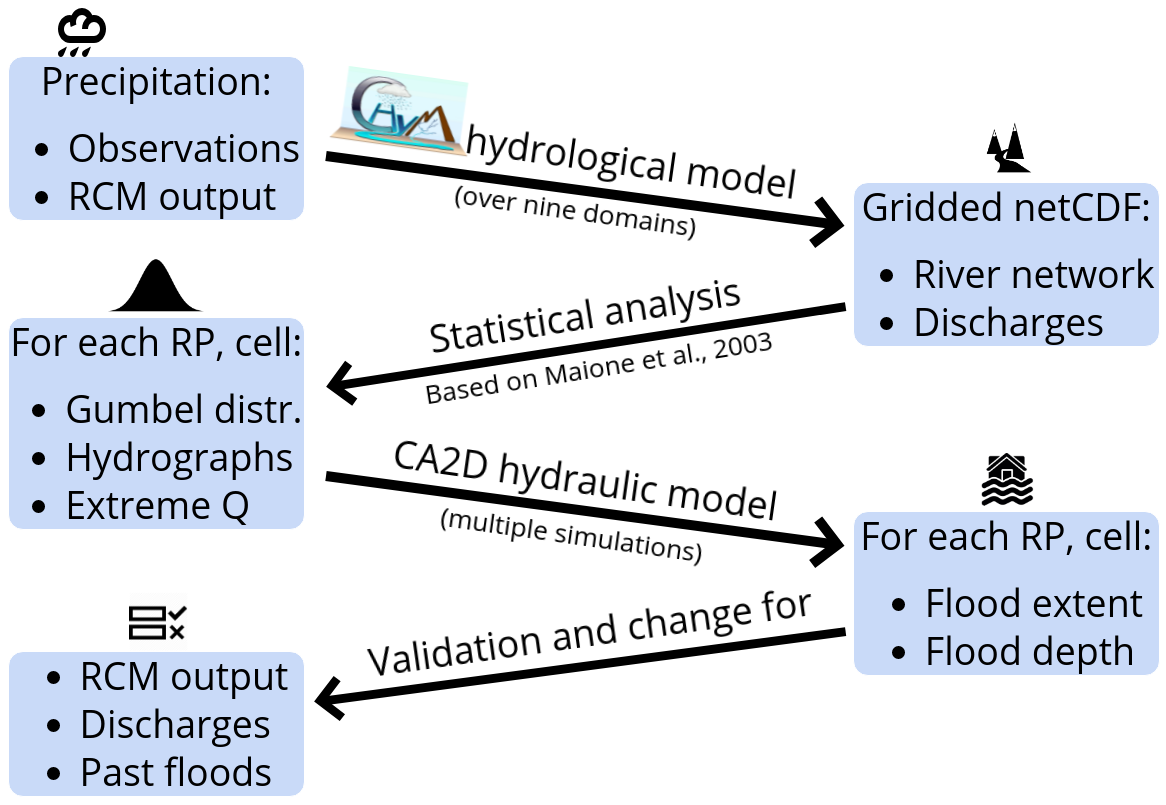
\includegraphics[width=\textwidth]{figures/method}
    \decoRule
    \caption[Flowchart of the project methodology]{A schematic description of the methodology employed in this study.}
    \label{fig:method}
\end{figure}

The precipitation data that are the main input needed to run hydrological simulations come from two different sources:
\begin{description}
    \item[High-resolution observations] the GRIPHO dataset, described in \cref{chp:itaobs}, which provide high-resolution hourly precipitation data.
    \item[Regional Climate Model simulations] two climate simulations, one run in perfect boundary mode and one with a climate projection.
\end{description}

\Cref{sec:regcm} will detail the RCM model and simulations, while \cref{sec:chym} will describe the hydrological model of choice and its three simulations.
\Cref{sec:3_mod_apprach} will delineate the statistical procedure used to derive the extreme discharge statistics from the discharge timeseries. Finally, \cref{sec:ca2d} will present the hydraulic model and its simulations.


%------------------------------------
%	REGCM
%------------------------------------

\section{The RegCM Regional Climate Model} \label{sec:regcm}
The ICTP RegCM is a Regional Climate Model developed at the ICTP and maintained primarily by Graziano Giuliani. The project is under very active development and new features, options and schemes are routinely added. RegCM is used by several institutions and research groups worldwide.\\
The RegCM model was the first limited area model to be developed for long-term climate simulations \citep{dickinson1989regional, Giorgi1989}. The model went through the second \citep{Giorgi1993}, third \citep{Pal2007} and fourth \citep{giorgi2012RegmoddespretesovemulCORdom} major revisions and is currently at version 4.7.0.\\
RegCM is a compressible, terrain-following sigma-vertical coordinate model, offering a large selection of physical parameterisations. The dynamics are essentially the same as the NCAR Mesoscale Model 4 or 5, depending on the versions and settings \citep[MM4, MM5,][]{Grell1994}.
Recently, the implementation of a non-hydrostatic core from MM5 has allowed to run in convection-permitting mode.
RegCM is mainly written in the Fortran programming language and is compliant with the Fortran 2003 ANSI standard; as most other climate models do, RegCM reads and writes files in the netCDF format.

\subsection{Regional Climate Models: an overview}
Regional Climate Models (RCMs) are Limited Area Models (LAMs) usually nested on larger datasets. RCMs are the most common tool used to ``zoom in'' on a specific area by dynamically \emph{downscaling} lower-resolution climate data. They do this by processing the information provided by the driving dataset at the domain boundaries, adding value thanks to the higher resolution and consequent more accurate representation of physical processes.\\
The first Regional Climate Models were initially developed in the late ´80s \citep{Giorgi1990, dickinson1989regional, Giorgi1989} to perform short, few-days simulations at best. In subsequent years, their use was extended to perform multi-year simulations \citep{Giorgi1993, Jones1995}. In the last two decades, several research programs utilising RCMs were put forward to advance the knowledge of climate at small spatial scales: of these, the most recent is the Coordinated Regional Climate Downscaling eXperiment (CORDEX, \cref{sec:cordex}).\\
In the nesting regional climate modelling technique, large scale (atmospheric and oceanic) time-dependent fields drive a higher resolution model over a limited domain. The driving data acts as boundary condition to the driven model and provides the initial conditions. In most cases a one-way nesting scheme is used: the nested model does not influence the boundary driving data, i.e.\ there is no feedback from the nested model to the coarser model. However, two-way coupled simulations, in which feedback from the driven model is incorporated in the boundary conditions, can be performed with some models \citep{Inatsu2009, Lorenz2005}.\\
By design, RCMs necessitate of external forcings that act as boundary conditions. These are usually of three kinds:
\begin{itemize}
    \item Model \emph{reanalysis}, such as ERA-Interim \citep{Dee2011}, are weather model simulations of the past which are constrained by a plethora of observed quantities through a complex process of data assimilation. The resulting dataset is uniform in time and space, consistent with observations, physically coherent, and provides all the necessary variables to drive an RCM. Such ``perfect boundary condition'' simulations are usually performed to validate the ability of an RCM to reproduce a reliable climate.
    \item Global Climate Models (GCMs) are physical simulations of the general circulation, much like RCMs, however with global extent and, thus, no external forcing other than the initial conditions. GCMs are the most natural choice for long climate projections; they usually have a resolution which, due to computational constraints, is significantly lower than that of RCMs.
    \item RCMs themselves can be used as driving data for even higher resolution simulations, in what is usually called a multi-nesting simulation. Such simulations are becoming more and more common thanks to the development of convection-permitting models \citep{Prein2015, Clark2016}, which often have a resolution of \SI{2}{\kilo\meter} or less and require high-resolution driving data.
\end{itemize}
Due to the presence of lateral boundary conditions, RCMs necessarily need to take into consideration  a so-called \emph{buffer zone}: a number of cells close to the domain edge in which the dynamical equilibrium between the driver and the driven model can be reached and smaller-scale features can develop. The same is true for an initial \emph{spin-up} period, usually of up to one or two years, which is excluded from analysis.

\subsection{The CORDEX project}\label{sec:cordex}
In order to properly validate whether climate models perform well, and whether RCMs add value to GCMs and reanalysis, a large number of ensemble simulations, performed on common domains, is advisable. Several  international projects have historically provided the basis for this kind of analysis. Some of these are PIRCS, START, CECILIA,
CLIM-RUN, MICE, STARDEX, PRUDENCE, SPECS, EUPORIAS, ENSEMBLES, and CORDEX. CORDEX\footnote{CORDEX stands for Coordinated Regional Climate Downscaling eXperiment} \citep{Giorgi2009, Gutowski2016, Giorgi2015}, a World Climate Research Programme (WCRP) sponsored project, is a framework for downscaling a large number of GCMs using both dynamical and statistical downscaling techniques. 14 common domains are specified (Africa, MENA, North, Central and South America, Antarctica, Arctic, EURO, MED, Australasia, East, Central, South and South-East Asia), mostly covering areas from previous intercomparison projects, with pre-defined resolutions and projections. Two European domains are defined, one covering all of the continent \citep[][EURO--CORDEX]{Jacob2014} and one focusing on the Mediterranean \citep[][Med--CORDEX]{Ruti2016}. Institutions are asked to provide data with a grid resolution of around 12, 25 or \SI{50}{\kilo \meter}; as will be shown in \cref{sec:experiments}, the domain chosen in this work covers the EURO--CORDEX area (\cref{fig:euro_cordex}) at a resolution of \SI{12}{\kilo \meter}.

\begin{figure}
    \centering
    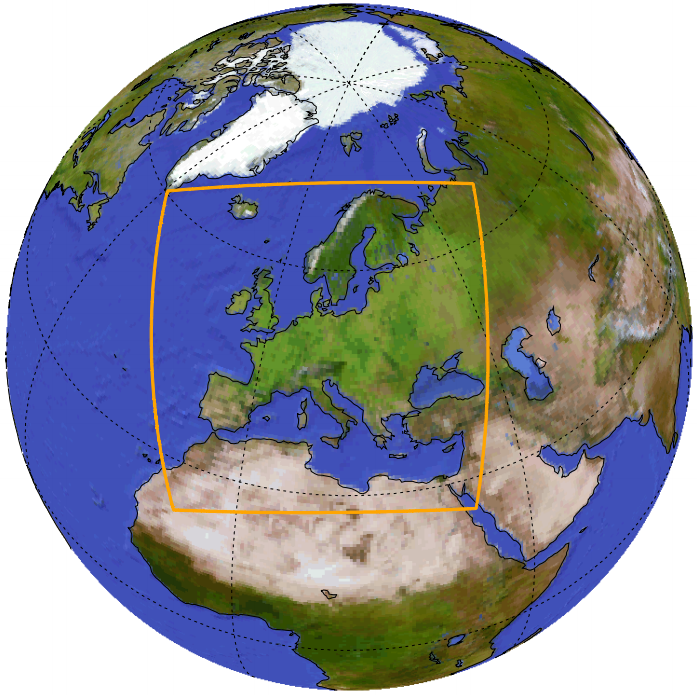
\includegraphics[width=0.7\textwidth]{figures/eurocordex}
    \decoRule
    \caption[EURO--CORDEX domain]{The approximate EURO--CORDEX domain, from \url{http://www.cordex.org/domains/cordex-region-euro-cordex/}} \label{fig:euro_cordex}
\end{figure}

\subsection{Added value of RCMs}
Why use Regional Climate Models, when Global Climate Models are a ever-improving, tried-and-tested approach to simulating climate?
The answer is that, even with today's increasingly powerful computational resources, GCMs are still run at a resolution of several tens of kilometers: for example, the latest Coupled Model Intercomparison Project 6 \citep[CMIP6,][]{Eyring2016} includes the High Resolution Model Intercomparison Project \citep[HighResMIP,][]{Haarsma2016}, whose simulations are supposed to run with a resolution of ``at least \SI{50}{\kilo \meter}''.
By contrast, \emph{convection-permitting} RCM simulations with spatial resolutions close to that at which the hydrostatic approximation starts failing \citep[about \SI{10}{\kilo \metre}][]{giorgi1999InttospesecRegclimodrev} are not a rarity anymore \citep[e.g.][]{Prein2015, Clark2016, Coppola2018}.
Thanks to the increased resolution, the main added value of RCMs is connected with their ability to reproduce otherwise unattainable small scale features (\cref{fig:topo_av}).
This is possible because of the better representation of:
\begin{description}
    \item[Orographic forcing] Increased resolution means increased ability to represent slopes, peaks and valleys. Variables that show a pronounced elevation dependency, such as precipitation, temperature and wind speed, greatly benefit from higher ground resolution. This is especially true for complex mountain areas \citep[see e.g.][]{Giorgi1989, Fischer2014}.
    % \item[Parametrisations] Physical process parametrisation usually improves at higher resolution, thanks to smaller timesteps and pixel areas.
    \item[Direct representation of processes] Some parametrisations can be eliminated altogether at very high resolutions, opting instead for direct representation of the processes. This is the case with the already mentioned convection-permitting models, in which convection is resolved explicitly.
\end{description}
\begin{figure}
    \centering
    \begin{subfigure}{0.4\textheight}
%        \caption{}\label{fig:topo_av/a}
        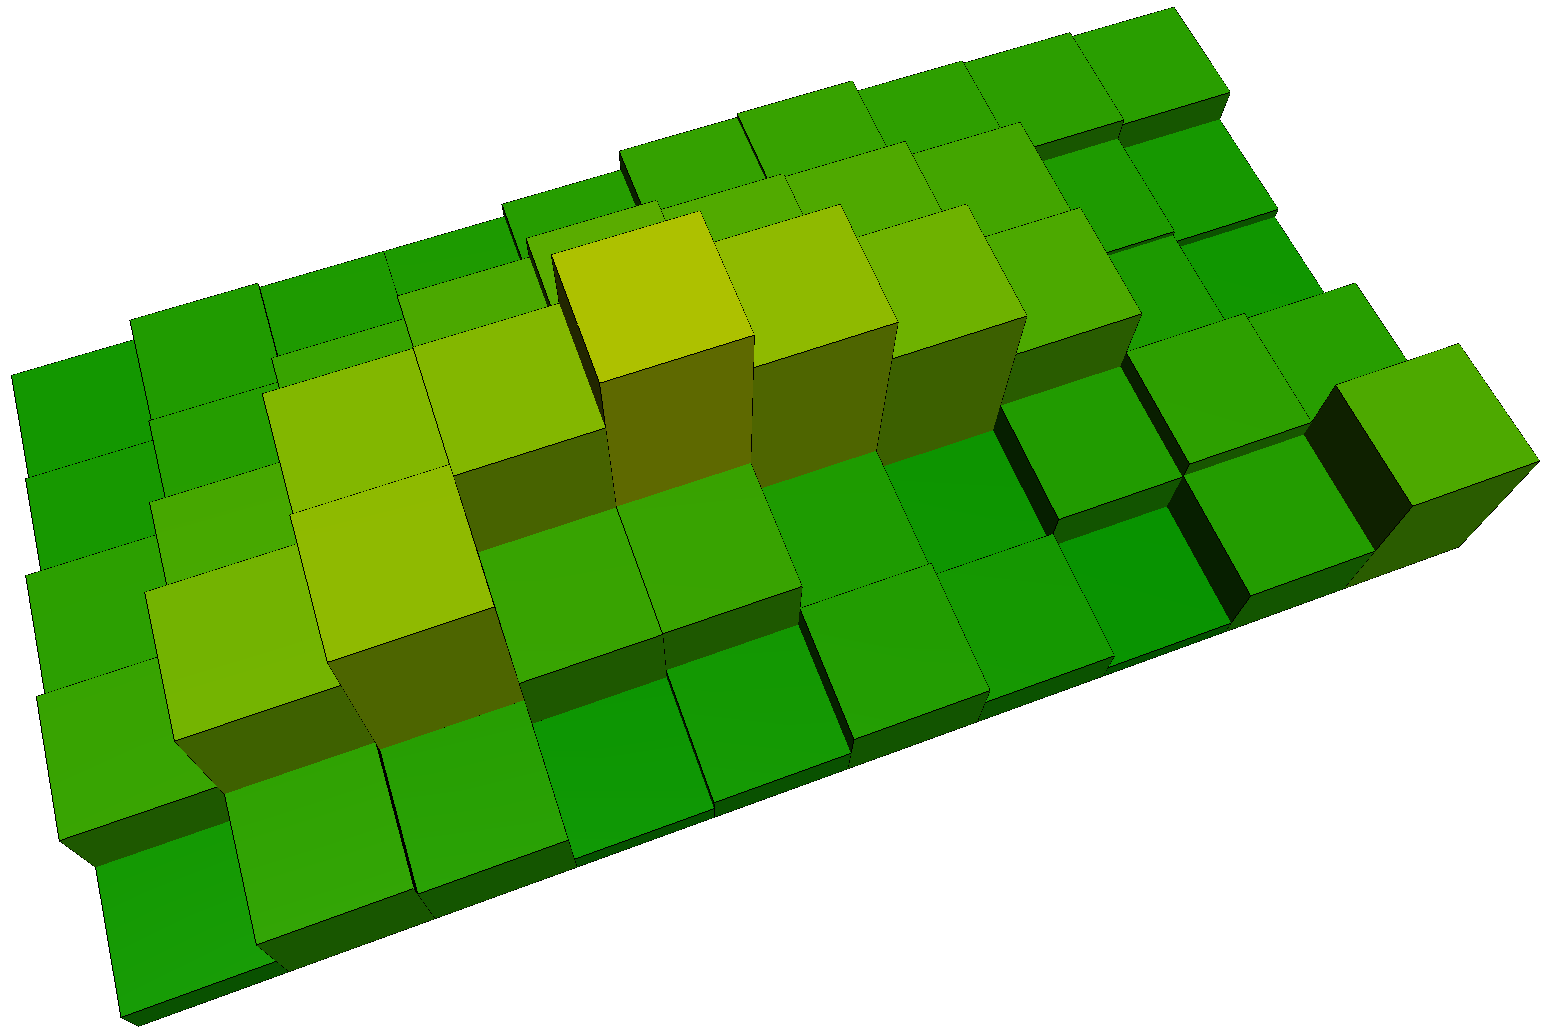
\includegraphics[width=\textwidth]{figures/topo_av/EI_3d}
    \end{subfigure}\\
    \begin{subfigure}{0.4\textheight}
%        \caption{}\label{fig:topo_av/b}
        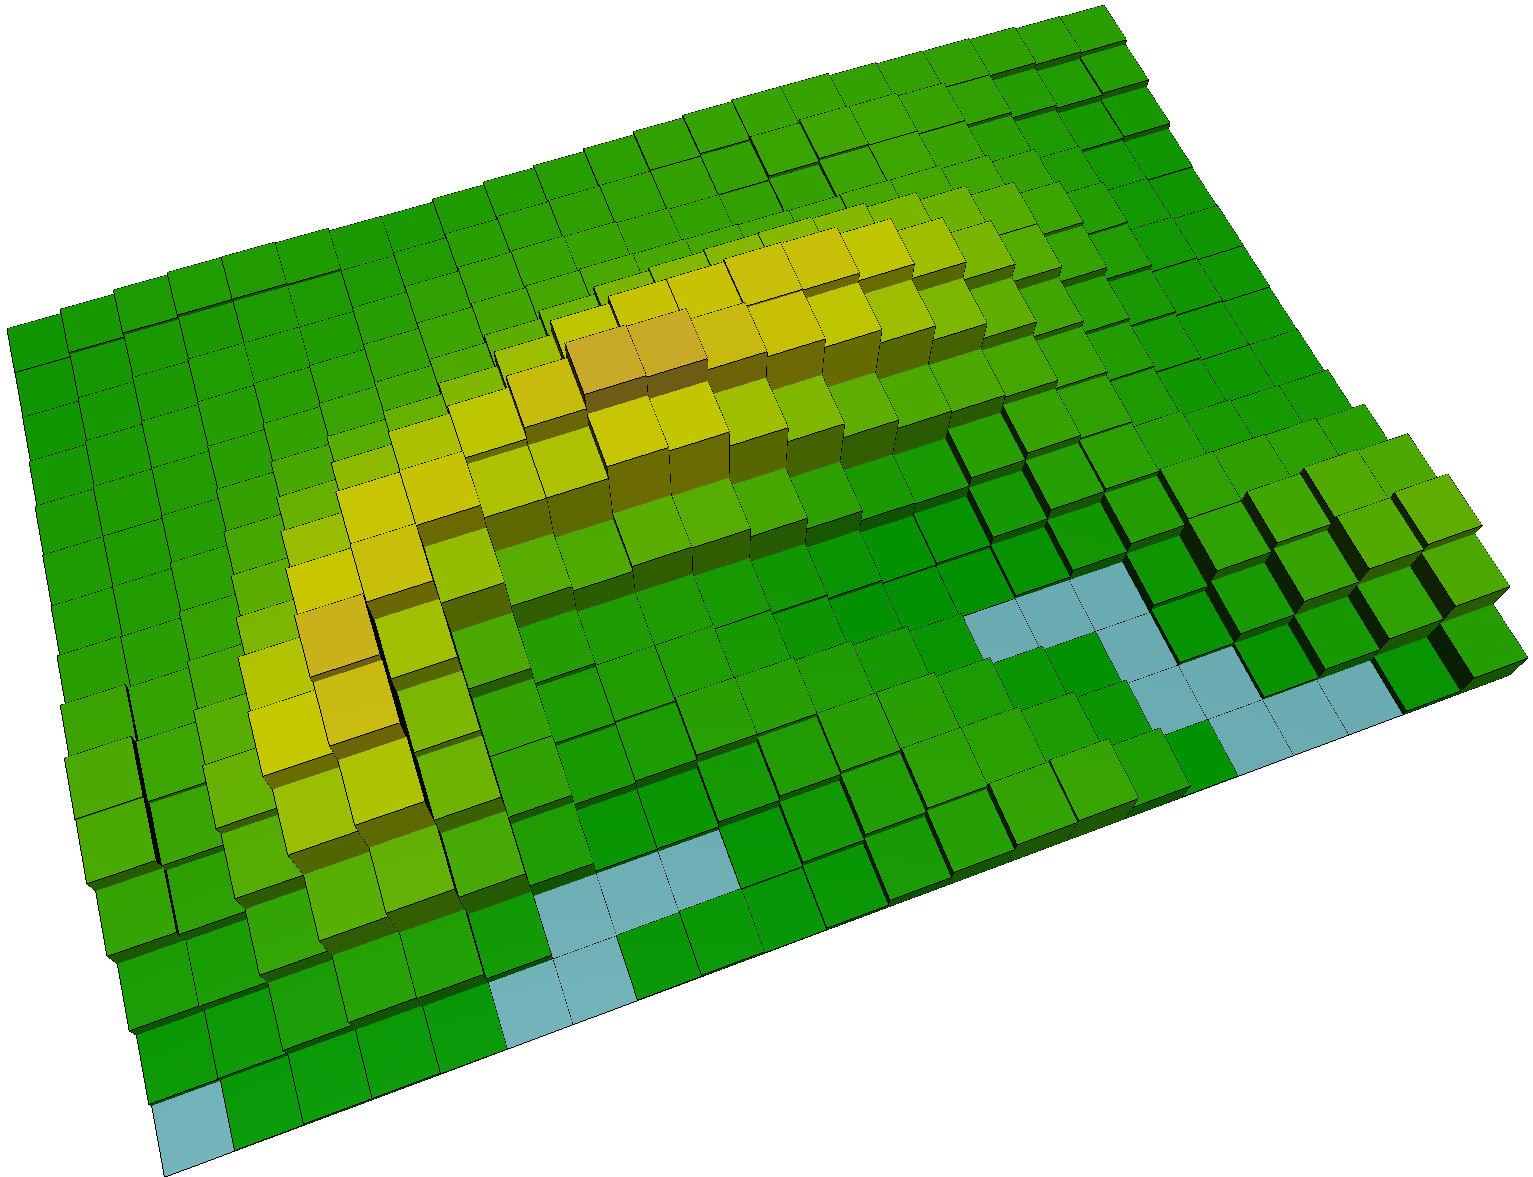
\includegraphics[width=\textwidth]{figures/topo_av/50_3d}
    \end{subfigure}\\
    \begin{subfigure}{0.4\textheight}
%        \caption{}\label{fig:topo_av/c}
        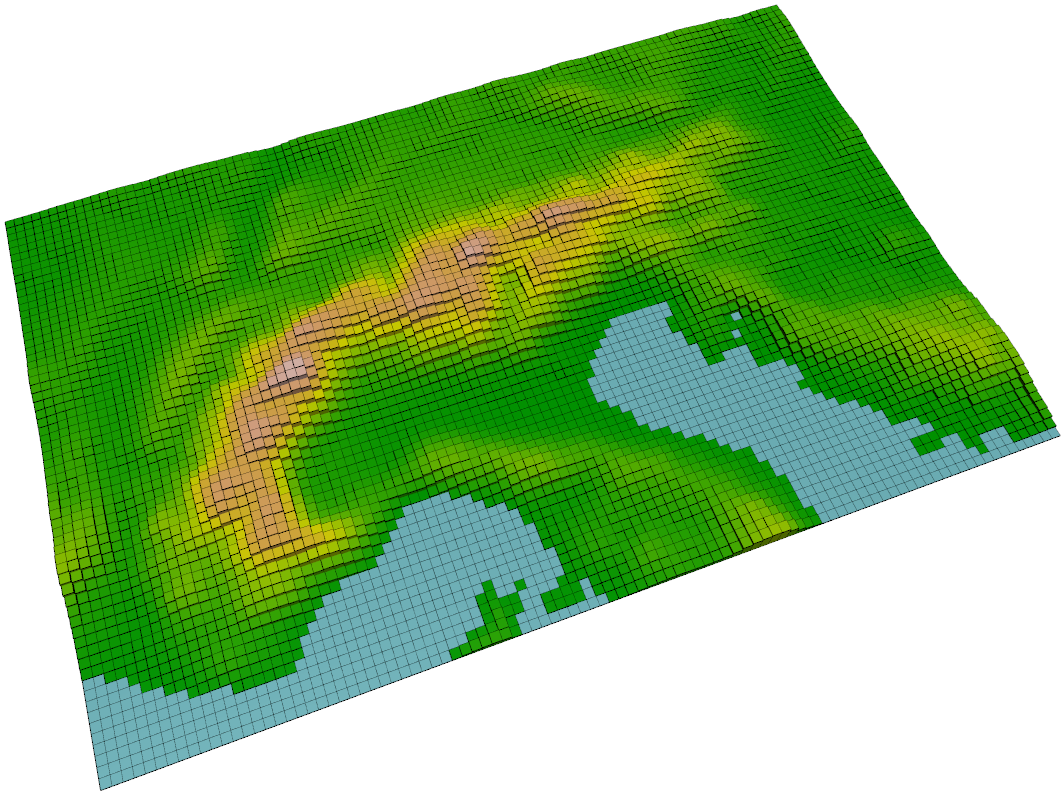
\includegraphics[width=\textwidth]{figures/topo_av/12_3d}
    \end{subfigure}
    \decoRule
    \caption[Topography representation over the Alps at different resolution]{
        Representation of topography over the Alps at different resolutions: \ang{1.50}, \ang{0.44} and \ang{0.11}, corresponding to the typical resolutions of GCMs, low-res RCMs and high-res hydrostatic RCMs respectively.
    }\label{fig:topo_av}
\end{figure}

RCMs, thus, usually add information to the global models which they are driven, if there are available observations of sufficient quality and resolution to assess this. This added information, if correct, is referred to as ``Added Value''.
It may seem obvious that increasing the resolution will improve the skill in reproducing climate.
However, added value is often hard to predict and identify, as it does not vary linearly with grid size nor is equal on different domains. As the IPCC \citep[][section 9.6.3]{IPCC2013} puts it:
\blockquote{
Although there are indications that model skill increases with higher resolution, it does not do so linearly. \citet{Rojas2006} found more improvement when increasing resolution from 135 km to 45 km than from 45 km to 15 km. \citet{Walther2013} found that the diurnal precipitation cycle and light precipitation improved more when going from 12 km to 6 km resolution than when going from 50 km to 25 km or from 25 km to 12 km. Higher resolution does enable better simulation of extremes \citep{Seneviratne2012}. For example, \citet{Pryor2012} noted that an increase in RCM resolution from 50 km to 6 km increased extreme wind speeds more than the mean wind speed. \citet{Kawazoe2013} compared six RCMs and the two GCMs to high resolution observations, concluding that precipitation extremes were more representative in the RCMs than in the GCMs. \citet{Vautard2013} found that warm extremes in Europe were generally better simulated in RCMs with 12 km resolution compared to 50 km. \citet{Kendon2012} and \citet{Chan2012} found mixed results in daily precipitation simulated at 12 km and 1.5 km resolution, although the latter had improved sub-daily features, perhaps as convection could be explicitly resolved.
}

Due to the importance of a reliable representation of extreme precipitation events for flood hazard, the added value that high resolution can provide for this variable deserves greater attention.
In a recent study, \citet{Fantini2016} compared 9 EURO-- and Med--CORDEX RCMs against high resolution regional observations for several metrics, of which two are extreme precipitation metrics.
The performance of the models was assessed at two different resolutions (\ang{0.11} and \ang{0.44}).
In most regions, the higher resolution RCMs showed better ability to reproduce extreme precipitation compared to the lower resolution ones: in the daily precipitation Probability Density Functions  (\cref{fig:added_value_pdf}), for example, the only case in which the performance was clearly degraded (when going from the \ang{0.44} to the \ang{0.11} ensemble) also coincided with the region characterised by the lowest density of stations (the Carpathians); other regions mostly showed better performance on part of the \ang{0.11} ensemble.
RCMs performed also significantly better than the driving ERA-Interim \citep{Dee2011} in all metrics (and in particular in extreme precipitation).\\
The results of this work are in general agreement, for what concerns extreme precipitation, with other similar works, such as \citet{diluca2012PotaddvalpresimbyhignesRegCliModobs, Lucas-Picher2017, Prein2016, Torma2015, Casanueva2016}, reinforcing the evidence supporting the presence of strong added value for extreme precipitation events in high-resolution RCM simulations.
\begin{figure}
    \centering
    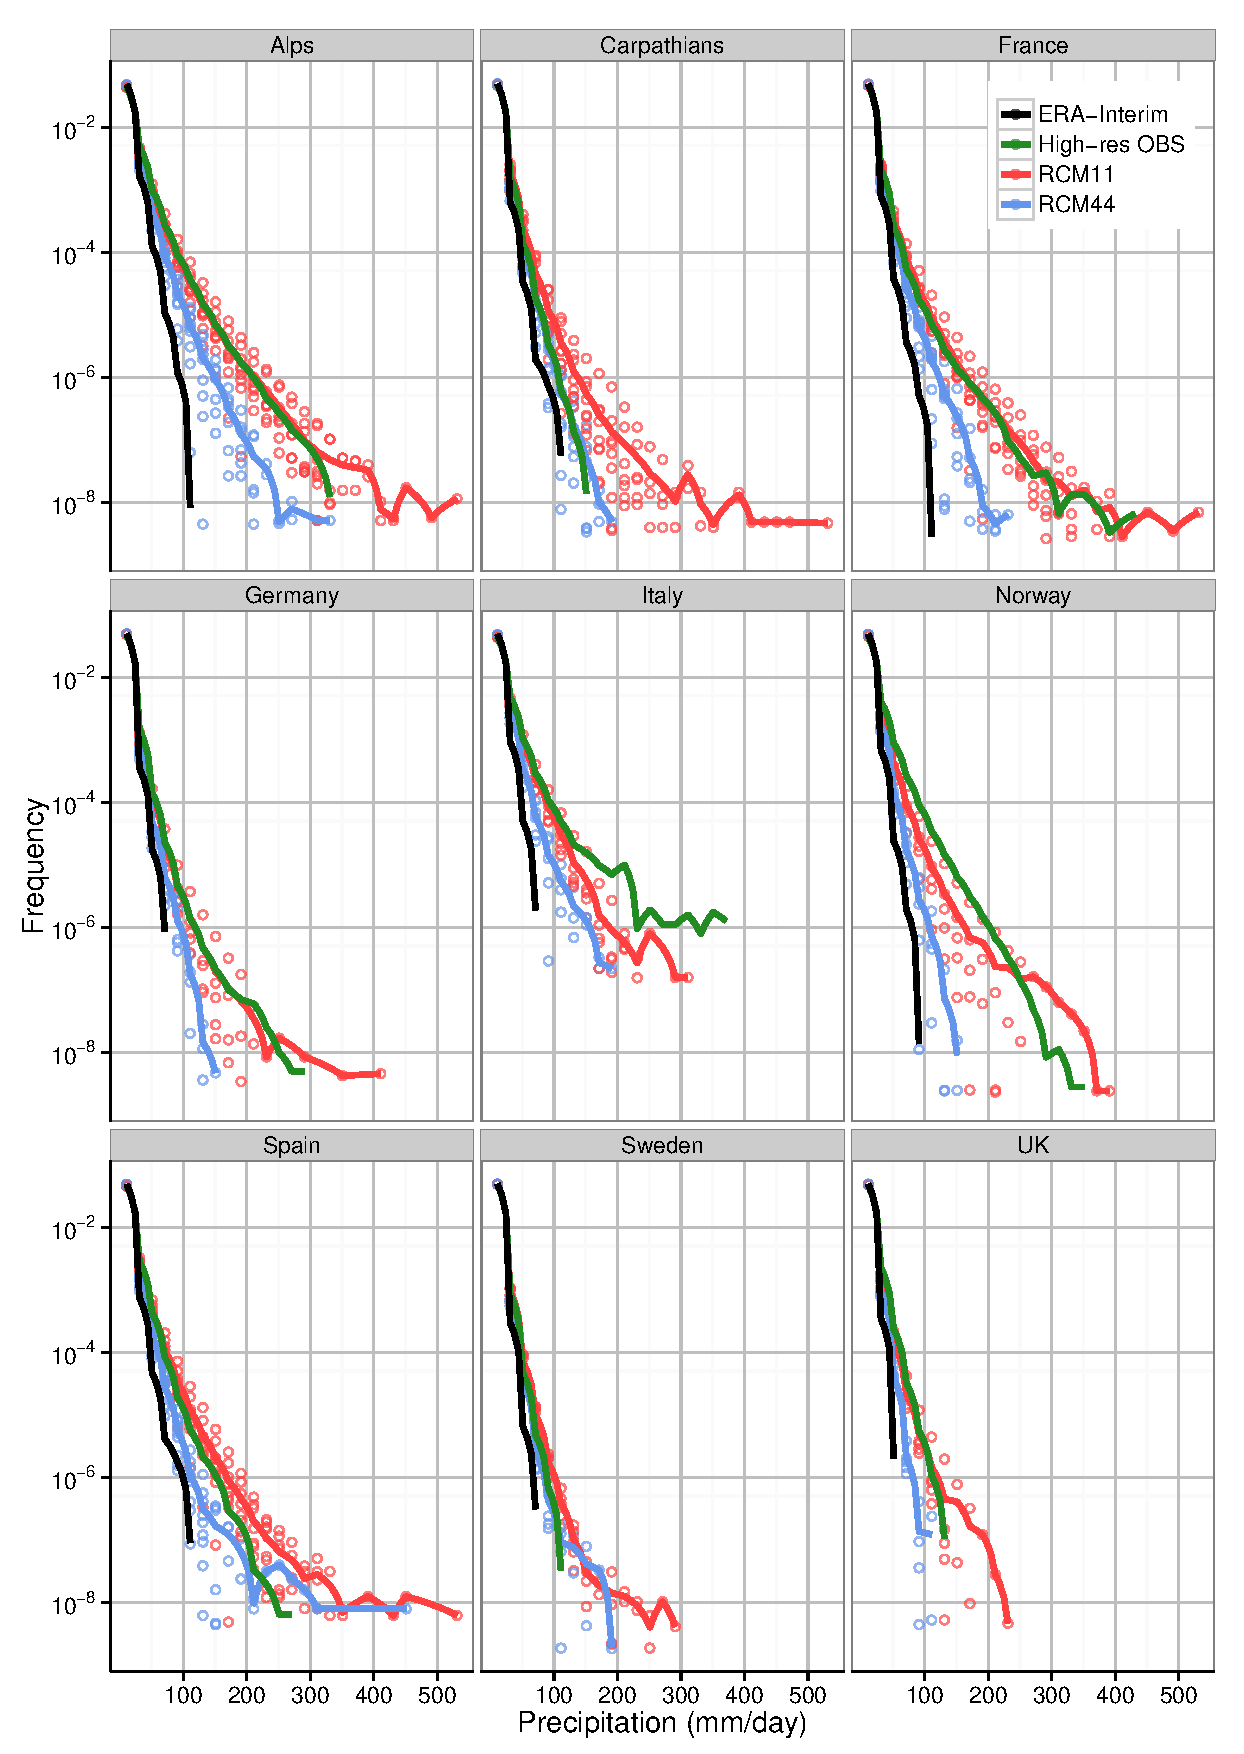
\includegraphics[width=\textwidth]{figures/AV_PDF}
    \decoRule
    \caption[PDFs for CORDEX models, from \citet{Fantini2016}]{Probability Density Functions (PDFs) for the ensemble average of the 9 models considered in \citet{Fantini2016} over the 9 regions where high-resolution observations were available. In black, the driving ERA--Interim data; in blue and red, the \ang{0.44} and \ang{0.11} ensembles respectively; in green the regional observations.} \label{fig:added_value_pdf}
\end{figure}
As a result of these considerations, the ICTP RegCM Regional Climate Model was selected to drive the hydrological simulations, both in the present day and in a future scenario. Due to limitations in time and computational resources, no additional model was selected to perform an ensemble simulation in order to reduce uncertainty; this, however, might be an interesting topic for future research.

\subsection{RegCM experiments}\label{sec:experiments}
In the framework of this thesis, two regional climate simulations with the ICTP RegCM Regional Climate Model are carried out, both on the complete European continent. One simulation is driven by the European Centre for Medium-range Weather Forecasts (ECMWF) ERA-Interim reanalysis \citep{Dee2011} and spans 1979--2016, the other is driven by the Met Office Hadley Centre HadGEM2 CMIP5 Global Climate Model \citep{Collins2011} and covers the period 1971--2099, under the IPCC Representative Concentration Pathway
8.5 \citep[RCP8.5,][]{IPCC2008moss,Riahi2007}. This business-as-usual scenario represents the worst-case future, in which no climate change mitigation measures are taken. This second simulation is part of the PRINCIPLES\footnote{Producing RegIoNal ClImate Projections Leading to European Services, \url{https://www.gerics.de/science/projects/detail/071974/index.php.en}} project.

In order to avoid the several pitfalls in defining a domain and to keep the simulation within the CORDEX project, the EURO-CORDEX domain (\cref{fig:euro_cordex}) was chosen, with a model resolution of \SI{12}{\kilo\meter} on a Lambert Conformal Conic projection. RegCM has been run on this domain before, so no adjustment to the domain position, size, and resolution was needed.
The initial testing started with the tagged version 4.5.0, but, after subsequent versions were released, the latest (at the time of starting the runs) RegCM 4.6.1 was selected for both simulations.

Model tuning was manually performed by simulating 3-year chunks and comparing them, after removal of a 1-year spinup period, with precipitation and temperature observations from the E-OBS dataset \citep{Haylock2008}.
In the case of the simulation driven by the ERA-Interim reanalysis, the first one to be submitted, 92 different tests had to be performed before choosing the final configuration.
The simulation driven by HadGEM2, which was started later and whose tuning started off of the first simulation's parameters, required 43 calibration iterations\footnote{
After the testing phase and the simulation of the historical period, James Ciarlo` from the Earth System Physics (ESP) section of the International Centre for Theoretical Physics (ICTP), took charge of the RegCM simulation driven by HadGEM. Thanks James!
}.\\
The first simulation ran on the ICTP ARGO cluster\footnote{\url{http://argo.ictp.it/}} using, on average, 200 processors, for a total actual runtime of about 2500 hours (0.5 million core-hours) for its 38 years of simulation.
The second simulation, which extended to 2099 with about 130 years of simulation, was run on the CINECA MARCONI cluster\footnote{\url{https://www.cineca.it/it/content/marconi}} Skylake partition using an average of 816 processors per run, for a total actual runtime of about 3000 hours (2.5 million core-hours) and \SI{90}{\tera B} of disk usage before post-processing.\\
The analysis of the two RegCM simulations will be presented in \cref{sec:valid_regcm}.

%------------------------------------
%	CHYM
%------------------------------------

\section{The CETEMPS Hydrological Model CHyM} \label{sec:chym}
The CETEMPS Hydrological Model \citep[CHyM\footnote{\url{http://cetemps.aquila.infn.it/chym/}}, ][]{Tomassetti2005,Coppola2007} is a distributed (gridded) hydrological model which simulates surface water runoff,
evapotranspiration, percolation, infiltration, melting and return flow.
The model uses information from a Digital Elevation Model (\cref{sec:DEM}) to reconstruct a D8 river network employing cellula automata algorithms \citep{Coppola2006,Coppola2007}, and works by assimilating input precipitation from different sources.
Routing water through each grid cell is achieved using continuity
and momentum equations based on the kinematic shallow water wave approximation of \citet{Lighthill1955}.
The current implementation, provided the necessary input data (at least soil type, elevation, precipitation and temperature), can run on any domain and at any resolution.\\
CHyM was previously used for assessing the hydrological conditions of the Po basin under global warming \citep{coppola2014ChahydconPobasundglowar}, and
is currently used operationally\footnote{See \url{http://cetemps.aquila.infn.it/chym/newoper/}, where the current situation is updated daily} at the CETEMPS Center of Excellence to forecast potential floods using stress indexes \citep{Verdecchia2008,Tomassetti2005}.
The nine Italian domains on which CHyM is operationally run are the same that will be employed in this thesis.

Although part of the model database is stored in Fortran-style binary files, the model was recently updated by Fabio Di Sante and Graziano Giuliani to produce output in the netCDF format, which facilitates postprocessing and analysis.
In order to ease the simulation setup, analysis, and monitoring, several tools were put into place to postprocess CHyM output. These include:
\begin{itemize}
    \item a graphical tool named \emph{chymview} to quickly and effectively visualise simulation outcome;
    \item automatic tools for the submission of cluster jobs;
    \item parallel programs for the final postprocessing and rechunking of time-slice netCDF data, for fast reading of discharge timeseries.
\end{itemize}

\subsection{Domains and river networks}\label{sec:chym_riv_net}
The first step in simulating the hydrology of the Italian territory is the division in subdomains and the creation of a reliable and plausible river network for each region.
As mentioned in the previous section, Italy is already fully covered by nine operational CHyM domains, on which the model has already been run and calibrated over several years of operational work.
The domains cover, approximately:
\begin{itemize}
    \item the Po river basin
    \item Liguria
    \item Central Italy
    \item North-Eastern Italy
    \item Central-Southern Italy
    \item Calabria
    \item Sicily
    \item Sardinia
    \item Central-Northern Italy
\end{itemize}
\Cref{fig:chym_regions} shows the nine domains over the complete Italian territory; some overlap between the domains is necessary in order to include all basins of interest for each domain.
\begin{figure}
    \centering
    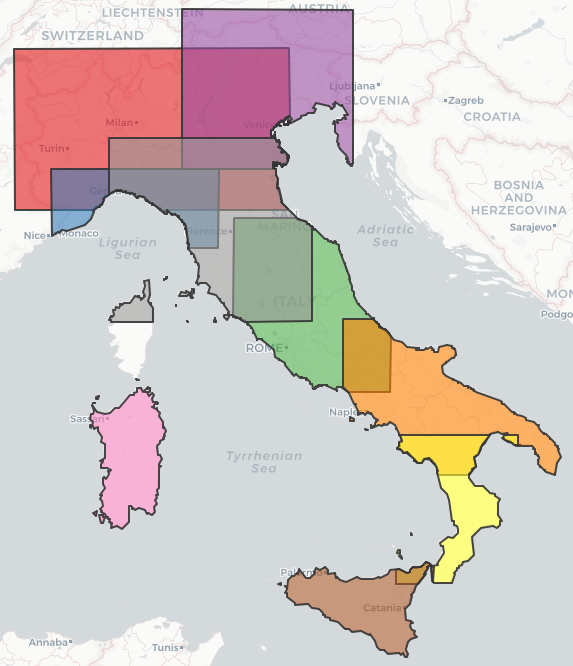
\includegraphics[width=0.6\textwidth]{figures/regions_crop}
    \decoRule
    \caption[The nine CHyM domains]{
        The nine domains on which the CHyM model is run operationally, which coincide with the domains used in this work.
    } \label{fig:chym_regions}
\end{figure}
The setup, resolution and physical configuration for each of the nine domains is different and based on the values suggested by CETEMPS; in particular, resolution ranges from about \SI{300}{\meter} (for Liguria, Calabria, Sicily and Sardinia) to about \SI{900}{\meter} (for the Po river domain).

Reproducing the river network for all domains represented a challenge.
CHyM uses several cellula automata algorithms to smooth the DEM, find no-flow spots, and connect them to the appropriate cells.
In this application, a reliable estimation of river network is crucial, in order to be able to assess inundation using the hydraulic model (see \cref{sec:ca2d}).
Initial tests with the default \SI{300}{\meter} Italian DEM shipped with CHyM did not lead to satisfactory results.
After further testing and tuning, we resorted to the HydroSHEDS hydrologically-conditioned DEM, which allowed for a more precise representation of river channels, thanks to the built-in river carving.
The configuration for the DEM smoothing and connection algorithms was tuned by automatically running several hundred preprocessing cycles with different parameters; the resulting river networks were then manually selected via an interactive web map (see \cref{fig:river_network} for an example).
Especially in the case of the Po plain, which is extremely flat and is simulated at a coarse resolution, the final reconstructed river network is within the limitations imposed by the resolution of the DEM.
Additional tests at an higher model resolution did slightly improve the river representation, but also increased the computational cost significantly.\\
Discharge stations (see \cref{sec:disch_obs}) have been manually repositioned on the simulated river network to insure proper comparison between model and observations.
\begin{sidewaysfigure}
    \centering
    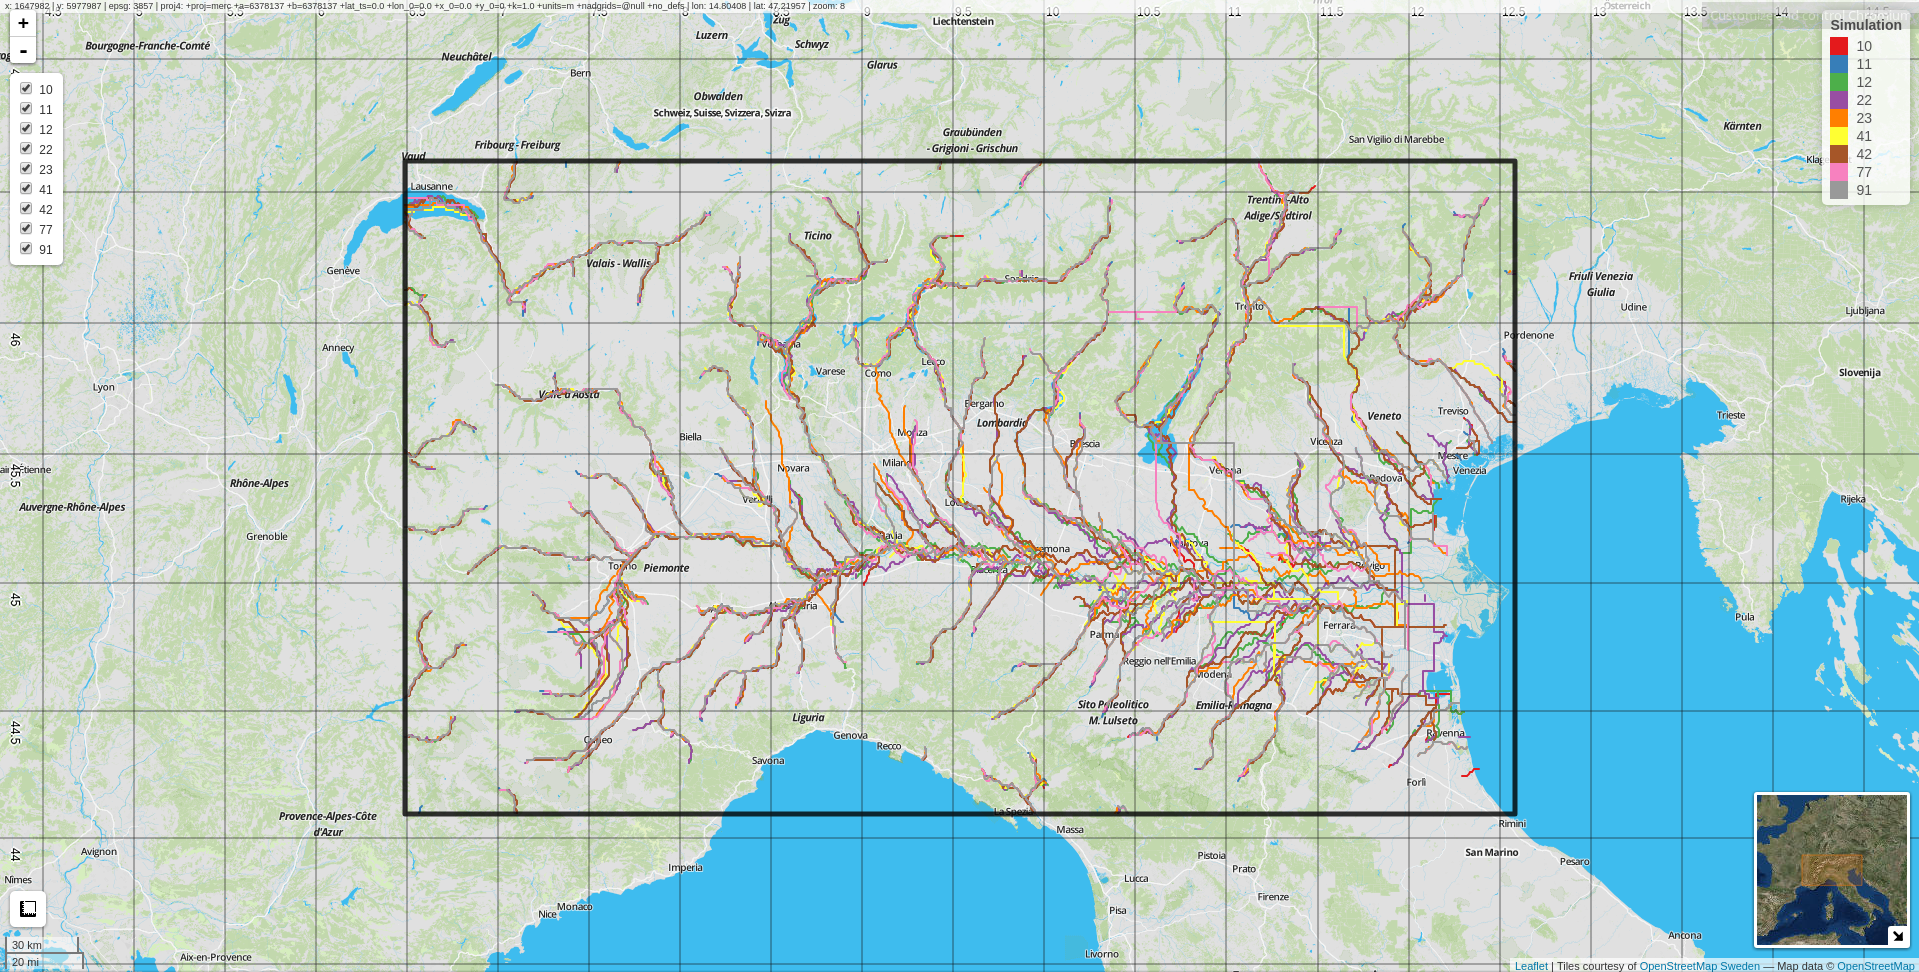
\includegraphics[width=\textheight]{figures/chym_routing_po}
    \decoRule
    \caption[Example river networks in the Po river basin]{
        Example of the river network creation experiments in the Po river basin. In order to obtain the most reliable representation of rivers, the candidate river networks are manually evaluated on top of a real world map.
    } \label{fig:river_network}
\end{sidewaysfigure}


\subsection{The three simulations}
Three CHyM simulations were run using the same configuration. They differed in the driving component: one was driven by the GRIPHO observational data presented in \cref{chp:itaobs}, one by the ERA-Interim-driven RegCM simulation, and one by the HadGEM-driven RegCM simulation (see \cref{tab:chym_sims}).
Each simulation was run on all the nine regions, for a total of 27 simulations.
GRIPHO's spatial and temporal coverage of the domains is not complete due to periods where station data is missing: the regions of Sicily and Puglia, in particular, are only covered for around 60\% of the timesteps over the 2001--2016 period.
For any timesteps and areas with missing data, daily weather forecasts performed with the operational MM5 model \citep{Grell1994} were used to fill in the gaps.
The MM5 model has been in use at CETEMPS for this particular purpose for almost two decades; for what concerns validation on the specific domain of application see, for example, \citet{Bianco2006}.

The computational requirements necessary to run CHyM are much lower than those of RegCM, but running on a cluster is still advisable.
The HadGEM-based simulation was run, similarly to its RegCM driver (see \cref{sec:experiments}), on the CINECA MARCONI cluster, while the other two simulations were run on the local ICTP ARGO cluster.
Although the CHyM model is parallel, its scaling is weak: for this reason, it was run limiting to one single compute node in both clusters (20 and 48 cores for ARGO and MARCONI SKL respectively).
However, the nine separate domains were run in parallel, effectively greatly reducing simulation time, which amounted in total to approximately 3000 runtime hours (or about 100000 core-hours) and almost \SI{35}{\tera B} of postprocessed output data.
\begin{table}[]
\centering
\begin{tabular}{@{}llll@{}}
\toprule
Driver              & Period     & Cluster & Disk usage \\ \midrule
Observations        & 2001--2016 & ARGO    & 5.6TB      \\
RegCM (ERA-Interim) & 1979--2016 & ARGO    & 7.2TB      \\
RegCM (HadGEM)      & 1971--2099 & MARCONI & 21TB       \\ \bottomrule
\end{tabular}
\caption{Details on the three CHyM simulations. The disk usage refers to the final usage of the postprocessed output.}\label{tab:chym_sims}
\end{table}

%------------------------------------
%	CLIMA-HYDRO-HYDRA APPROACH
%------------------------------------
\section{The climatological-hydrological-hydraulic approach} \label{sec:3_mod_apprach}
The flood hazard estimation method developed in this project follows the footsteps of similar approaches as illustrated in \cref{subs:flood_hazard_methods}: a hydrological model (\cref{sec:chym}), driven by observations (\cref{chp:itaobs}) or by a Regional Climate Model (\cref{sec:regcm}), reproduces discharge data over several different Italian domains and for a period of several years; these discharges are then fitted statistically to an extreme value distribution which allows to extend the simulation of extreme events to any Return Period, with decreasing accuracy as the rarity of the event increases.
The typical discharge for a selected number of Return Periods for each point is then modelled via a hydraulic model ((\cref{sec:ca2d})) to produce flood extent maps.
In our case, the statistical procedure, studied and devised by Francesca Raffaele from the ICTP's ESP section, is based on the work of \citet{Maione2003}, who present a procedure for the construction of ``typical'' flood discharge curves (called Synthetic Design Hydrographs) for any point of a river.
\citet{Maione2003} derive their methodology by estimating SDHs for gauged sites in the Po river basin, and extending the SDH definition to ungauged sites with a relation depending on the drained area.
This allows for a unique, consistent methodology to be applied across the whole catchment for every river cell --- in our case, the derivation of the SDHs is performed for every CA2D ``virtual station'' (see \cref{sec:ca2d}), starting from CHyM discharge data (\cref{sec:chym}).
In the following, the technical details and the formulae necessary to perform the calculations which result in the input data for the hydraulic model are described.

Given any river or station point, from model or observed data, the input to the statistical analysis is the complete timeseries of discharge for that specific location. Other than this, the analysis we performed is completely independent of location, albeit a few assumptions had to be made to generalise the process.\\
The aim is to obtain curves describing, for the given Return Period, the typical discharge timeseries of the event at that river point. These $Q_{RP}(t)$ curves will be called Synthetic Design Hydrographs (SDHs) and give the discharge ($Q$) of a typical extreme event as a function of the Return Period ($RP$) and the time ($t$).
SDHs are required by the hydraulic model (see \cref{sec:ca2d}) to simulate flood extent.

We start by defining the Flow Duration Frequency reduction curve (FDF) ($Q_D\left( RP \right)$, which is the discharge averaged over a duration $D$ (usually in hours) around the flood peak with Return Period $RP$.
As a consequence, the instantaneous FDF ($D=0$) represents the peak flood discharge $Q_0\left( RP \right)$.
The FDF is usually obtained from statistical analysis of historical hydrographs, but its formulation, as we shall see, can be generalised.

Similarly to the work of \citet{Maione2003}, we perform with the reasonable assumption that the reduction ratio ($\varepsilon_D$), which is the ratio of the FDF and the peak flood discharge ($Q_0\left( RP \right)$), is constant for any Return Period $RP$, so that:
\begin{equation}
  \varepsilon_D = \varepsilon_D\left( RP \right) = \frac{Q_D\left( RP \right)}{Q_0\left( RP \right)}\,,
  \end{equation} 
which means that the reduction ratio only depends on the duration $D$, as also reported by the \citet{NERC1975}.
As in \citet{Maione2003}, when performing the calculation of the FDF around each historical flood peak, the centring of the duration window of width $D$ is chosen as to maximise the average computed discharge $Q_D$:
\begin{equation}
  \text{FDF} = Q_D = \frac{1}{D} max \int_{t}^{t+D} Q \left(\tau \right) d\tau \,,
\end{equation}
where $t$ and $\tau$ represent time. Note that the product $Q_D \times D$ represents in fact the volume of water flowed in the duration $D$. The shape of the final synthetic hydrograph will be determined by the peak-duration ratio $r_D$: the ratio of the time before the peak and the total duration $D$ of the averaging window.
The smaller the $r_D$, the more skewed the hydrograph will be towards steeper (flatter) rising (falling) limbs of the hydrograph.
An example is given in \cref{fig:example_rd_maione}, which shows a possible high discharge event and the graphical representation of the FDF.

Centring on $t=0$ as the peak flood timing, the two limbs of the hydrograph can be described as:
\begin{equation}
  \int^{t=0}_{-r_DD} Q\left(\tau \right) = r_D D Q_D\left(RP \right)
\end{equation}
and
\begin{equation}
  \int^{\left(1-r_D\right)D}_{t=0} Q\left(\tau \right) = \left(1-r_D\right) D Q_D\left(RP \right) \,,
\end{equation}
where $Q_D\left(RP \right)$ is the typical FDF curve for the Return Period $RP$. The SDH is constructed imposing that the maximum discharges for each duration coincides with the value obtained from FDF curves. Differentiating with respect to $D$ we get, for the falling limb:
\begin{equation}\label{eq:sdh}
  \text{SDH} = Q_t \left( RP \right) = \frac{d/dD \left[ \left( 1-r_D\right) D Q_D\left(RP\right)\right]|_{D=D\left(t\right)}}{d/dD \left[ \left( 1-r_D\right) D \right]|_{D=D\left(t\right)}}\,,
\end{equation}
where $t=\left( 1-r_D\right)D$. Once the reduction ratio ($r_D$) and the FDF ($Q_D\left( RP\right)$) are known, this formula will allow to calculate the SDH.\\
\begin{figure}
    \centering
    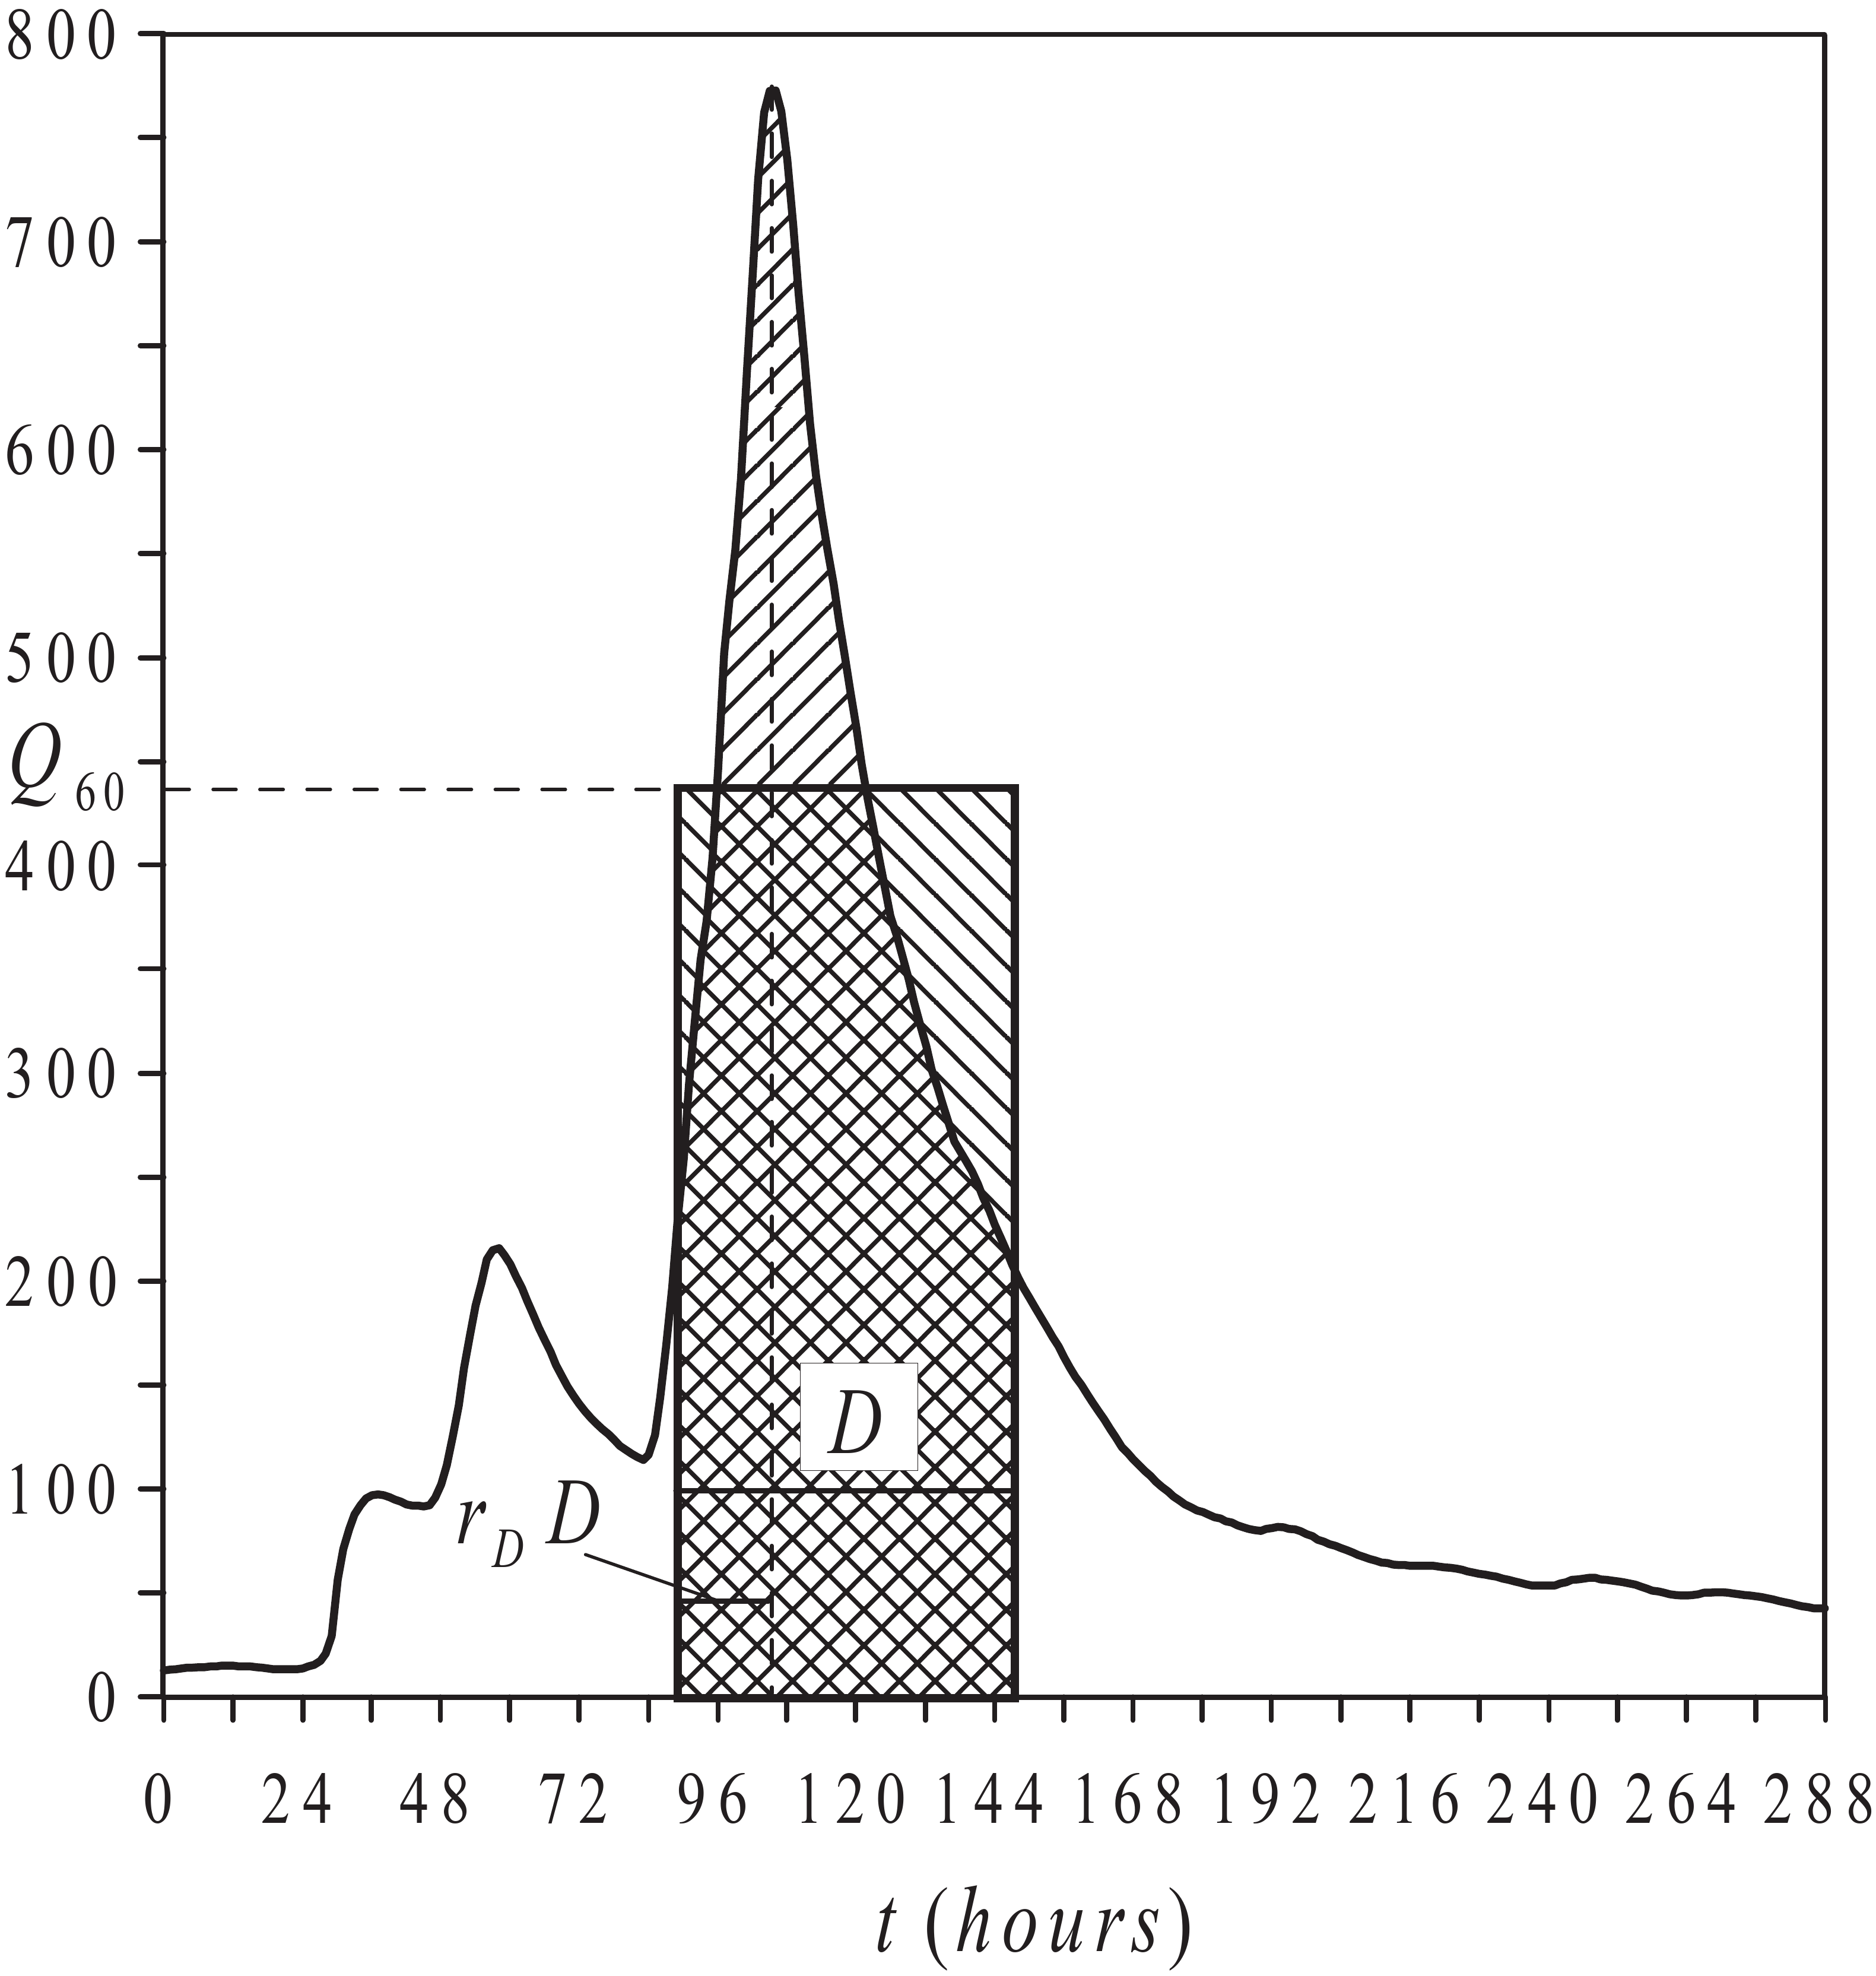
\includegraphics[width=0.5\textwidth]{figures/maione}
    \decoRule
    \caption[Example for the calculation of the Flow Duration Frequency curve]{
    Example for the calculation of the Flow Duration Frequency curve, from \citep[][figure 1]{Maione2003}. $D$ is the chosen duration (\SI{60}{\hour} in this image), $r_D$ the peak-duration ratio, $Q_{60}$ the value which maximises the integral of the discharge (or running average, for discrete data) for the given $D$.
    }\label{fig:example_rd_maione}
\end{figure}
In the context of this work, similarly to \citet{Alfieri2014}, we chose to assume symmetry of the hydrograph, that is:
\begin{equation}
  r_D = \frac{1}{2}\,,
\end{equation}
meaning that the duration windows are always centered on the flood peak and that the peak is in the centre of the hydrograph. Additionally, by definition, this also results in $t = \tfrac{1}{2} D$.\\
The maximum flood discharge $Q_0\left(RP\right)$ for any given Return Period $RP$ must then be calculated by fitting an appropriate extreme distribution. Following \citet{Maione2003, Alfieri2015a}, we chose the Gumbel distribution, so that:
\begin{equation}\label{eq:Q0fit}
  Q_0\left(RP\right) = u - \alpha \ln \left[ -\ln \left(1 - \frac{1}{RP} \right)\right] \,,
\end{equation}
where the parameters $u$ and $\alpha$ are estimated from the fit.
Given the timeseries of yearly discharge maxima $Q_y$, the parameters are estimated by fitting \cref{eq:Q0fit} for the selected Return Period, using the following initial parameters for scale ($\alpha$) and location ($u$):
\begin{equation}
  \alpha = \frac{\sqrt{6}}{\pi} \sigma\left(Q_y \right) \quad ; \quad u = \mu\left(Q_y\right) - \gamma \alpha \,,
\end{equation}
where $\gamma$ is the Euler-Mascheroni constant (equal to approximately 0.5772) and $\mu$ and $\sigma$ the mean and standard deviation operators respectively. Different fitting methods did not provide significantly different results in initial testing, so a simple maximum likelyhood method was selected.

We resort to the following approximation for the reduction ratio $\varepsilon_D$ :
\begin{equation}\label{eq:epsilon}
  \varepsilon_D \simeq \sqrt{p_2 \left[ 2 + p_1 - \frac{3}{2}p_2 \left(1 - p_1 \right) \right]} \,,
\end{equation}
where
\begin{equation}
  p_1 = e^{-4D/\theta} \quad \textrm{and} \quad p_2 = \frac{\theta}{2D}
\end{equation}
and $\theta$, the scale of fluctuation, is a parameter which, in our case, is considered to have a linear relationship with the drained area, as in \citet{Maione2003}. The approximation in \cref{eq:epsilon} is suited for large catchments; in this work, however, it is assumed to hold reasonably well for smaller basins.
Differentiating \cref{eq:sdh}, the falling limb of the SDH can be expressed as:
\begin{equation}
\begin{split}
  \text{SDH} = Q_t\left(RP\right) & = \frac{Q_o\left(RP\right) \left(p_2 - p_1 - p_2p_1\right)}{\varepsilon_D} \\ =
  & \frac{\lbrace u - \alpha \ln \left[ -\ln \left(1 - \frac{1}{RP} \right)\right]\rbrace \left(p_2 - p_1 - p_2p_1\right)}{\sqrt{p_2 \left[ 2 + p_1 - \frac{3}{2}p_2 \left(1 - p_1 \right) \right]}}
\end{split}
\end{equation}
This equation allows us to calculate a typical flood event discharge timeseries for any location and Return Period, starting only from the timeseries of yearly maximum discharges $Q_y$.

Tuning and testing for the method was carried over on the upper Po basin. The region was chosen due to previous experience with the hydrological model on this domain \citep{coppola2014ChahydconPobasundglowar}, availability of reliable observed discharge data, and lack of large water management structures.
Due to the relatively small size of the simulated domains, the calculation was carried over for durations up to \SI{240}{\hour}.
As highlighted, this approach requires some strong assumptions; the results however are reasonable despite these approximations.
Estimating and reducing the uncertainty deriving from the mentioned assumptions would certainly be a possible avenue for future work.
An example SDH, obtained from discharge data from the European Water Archive (see \cref{sec:disch_obs}) for a station on the Tevere river, is shown in \cref{fig:example_SHD}; \cref{fig:po_sdh} instead shows the SDHs for the seven discharge stations in the MV1 dataset (which covers the Po river, see \cref{fig:disch_dst}). The SDHs are similar to those produced by \citet{Maione2003}, indicating that the procedure is correct.

This procedure, as shown in the following chapters, was applied both with observational data and with data coming from a Regional Climate Model. 9 domains covering the complete Italian territory were simulated, but no limitation is in place that would prevent this technique to be applied to any domain worldwide. For each domain, a large number of small flood simulations was performed in order to cover all segments of the river courses.
\begin{figure}
    \centering
    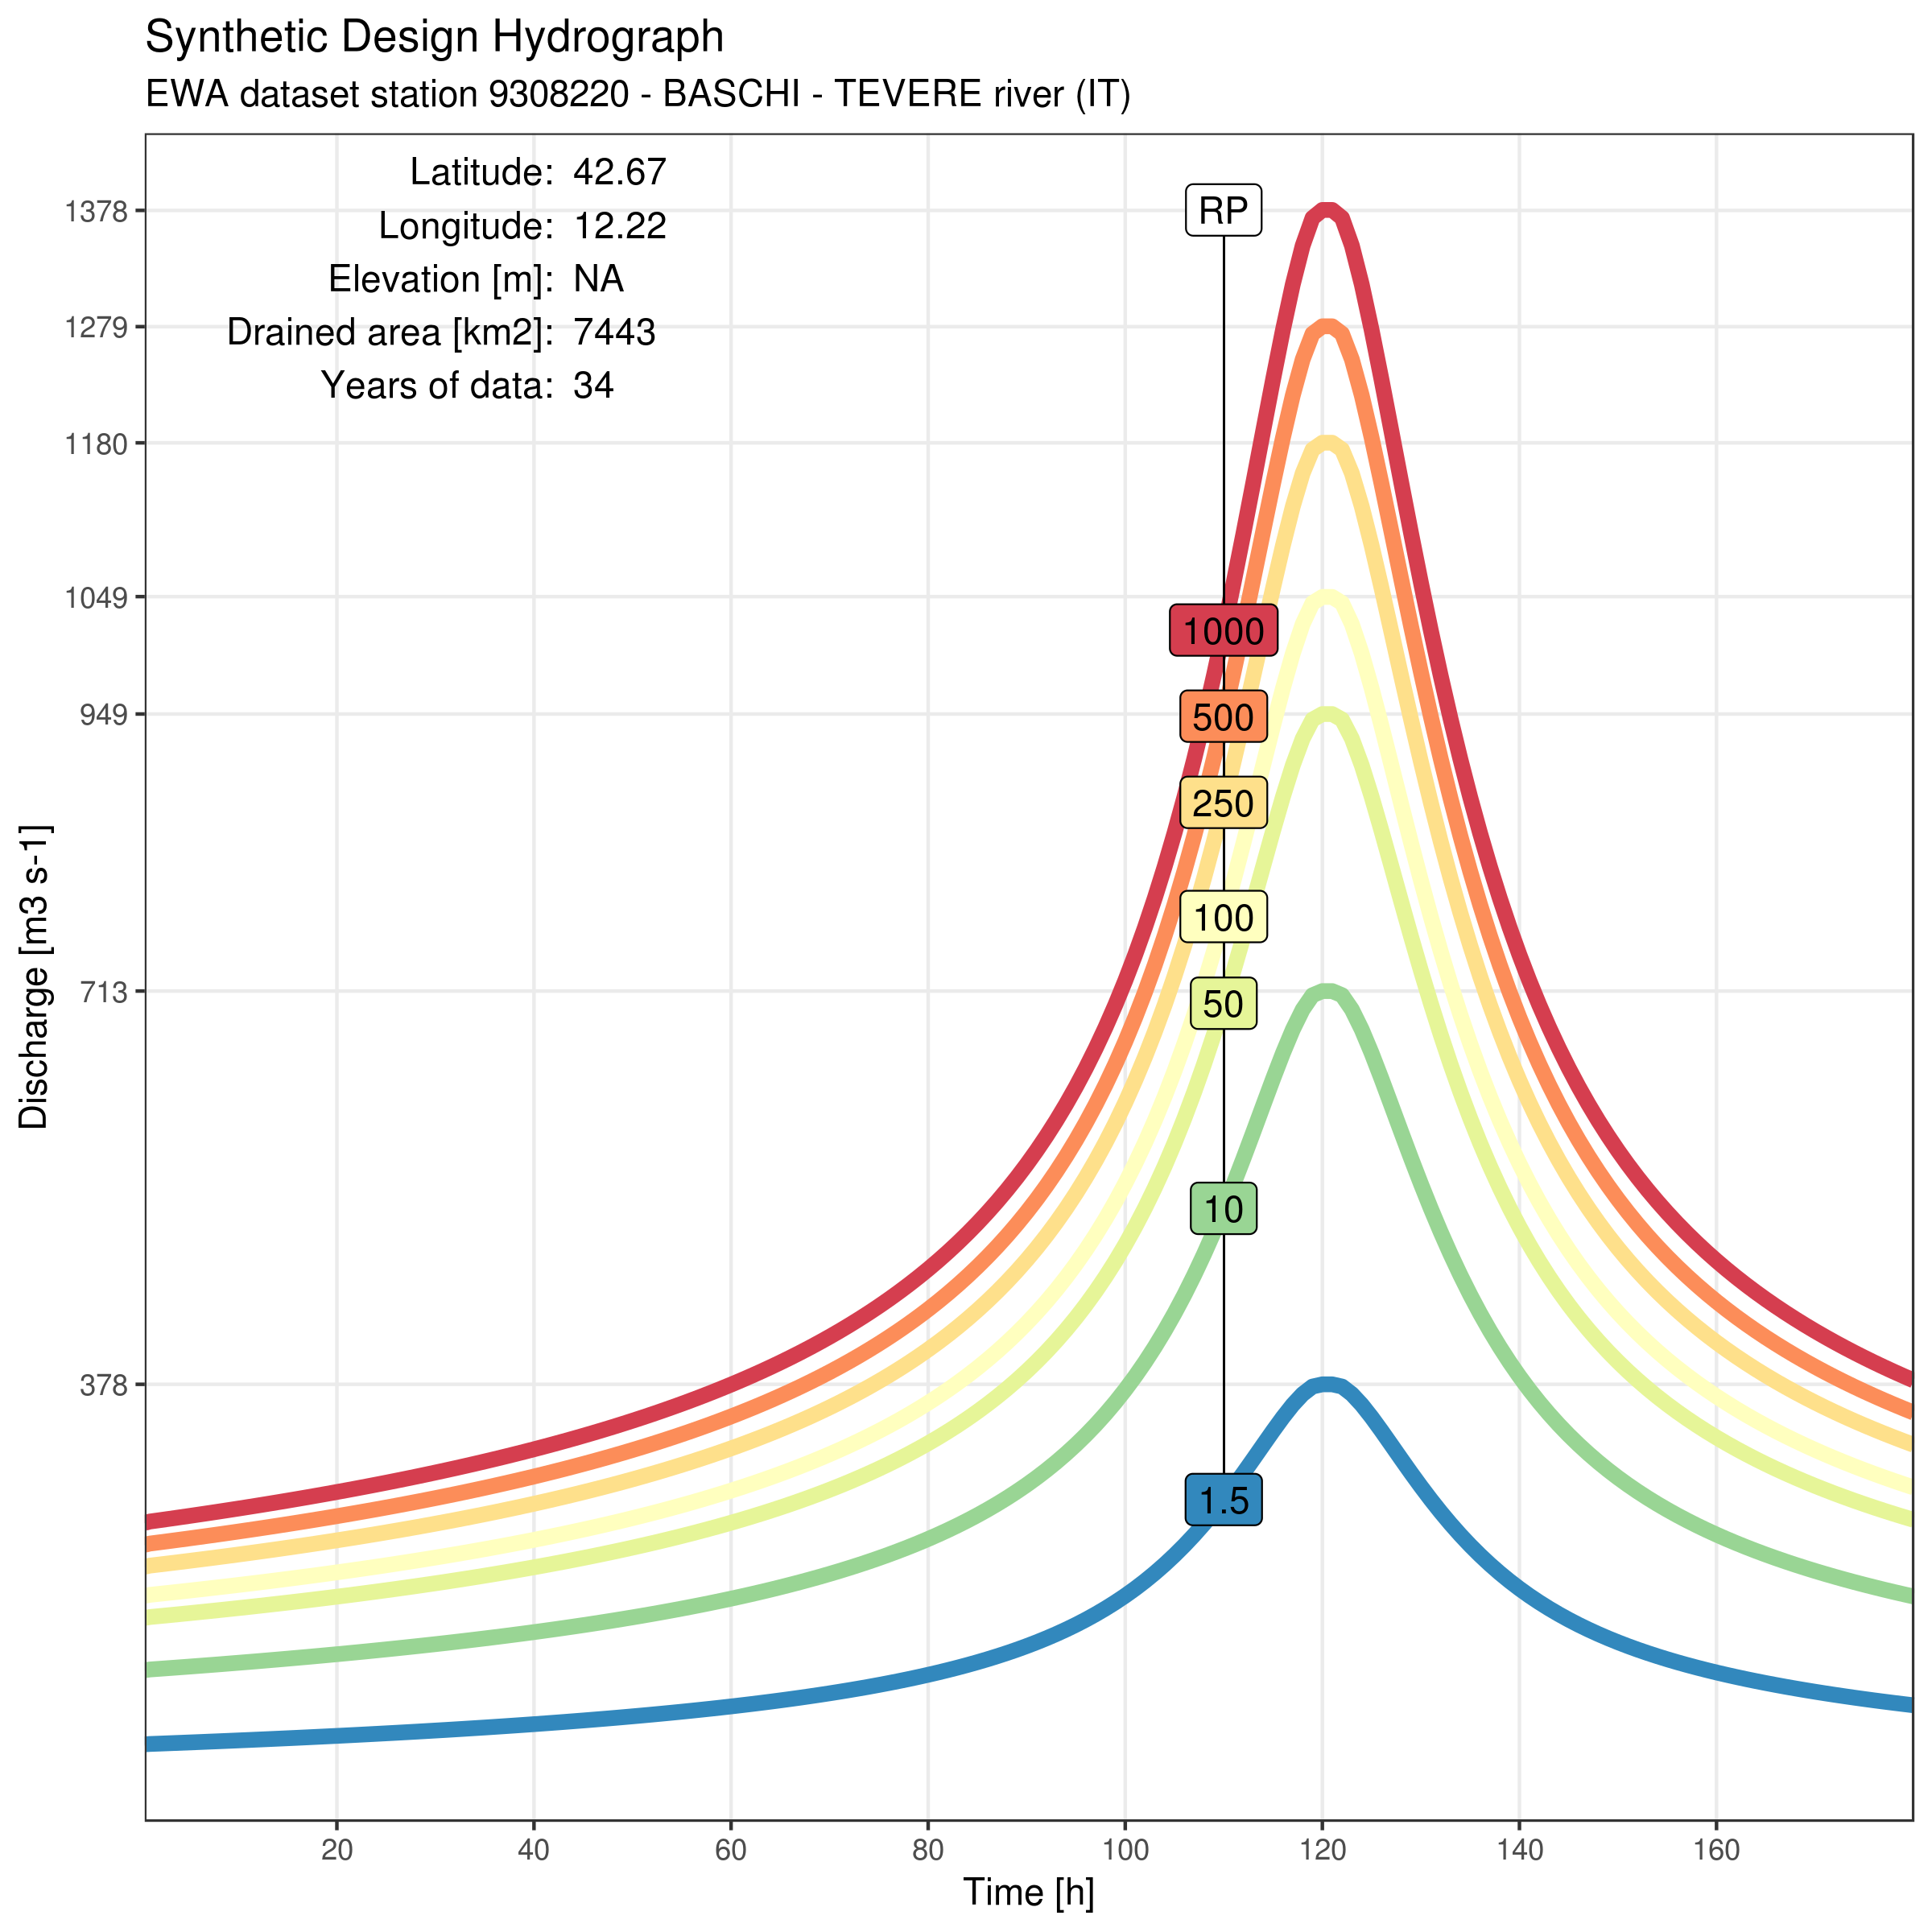
\includegraphics[width=0.7\textwidth]{figures/example_sdh}
    \decoRule
    \caption[Example Synthetic Design Hydrograph]{Example Synthetic Design Hydrograph computed following the procedure described in \cref{sec:3_mod_apprach} for a station on the Tevere River, in Central Italy. Seven Return Periods (1.5, 10, 50, 100, 250, 500 and 1000 years) are shown. Discharge data taken from the European Water Archive; see \cref{sec:disch_obs} for additional details.}
    \label{fig:example_SHD}
\end{figure}
\begin{figure}
    \centering
    % from /home/afantini/places/clima-archive/flood/museodat2nc/calc_SDHs/
    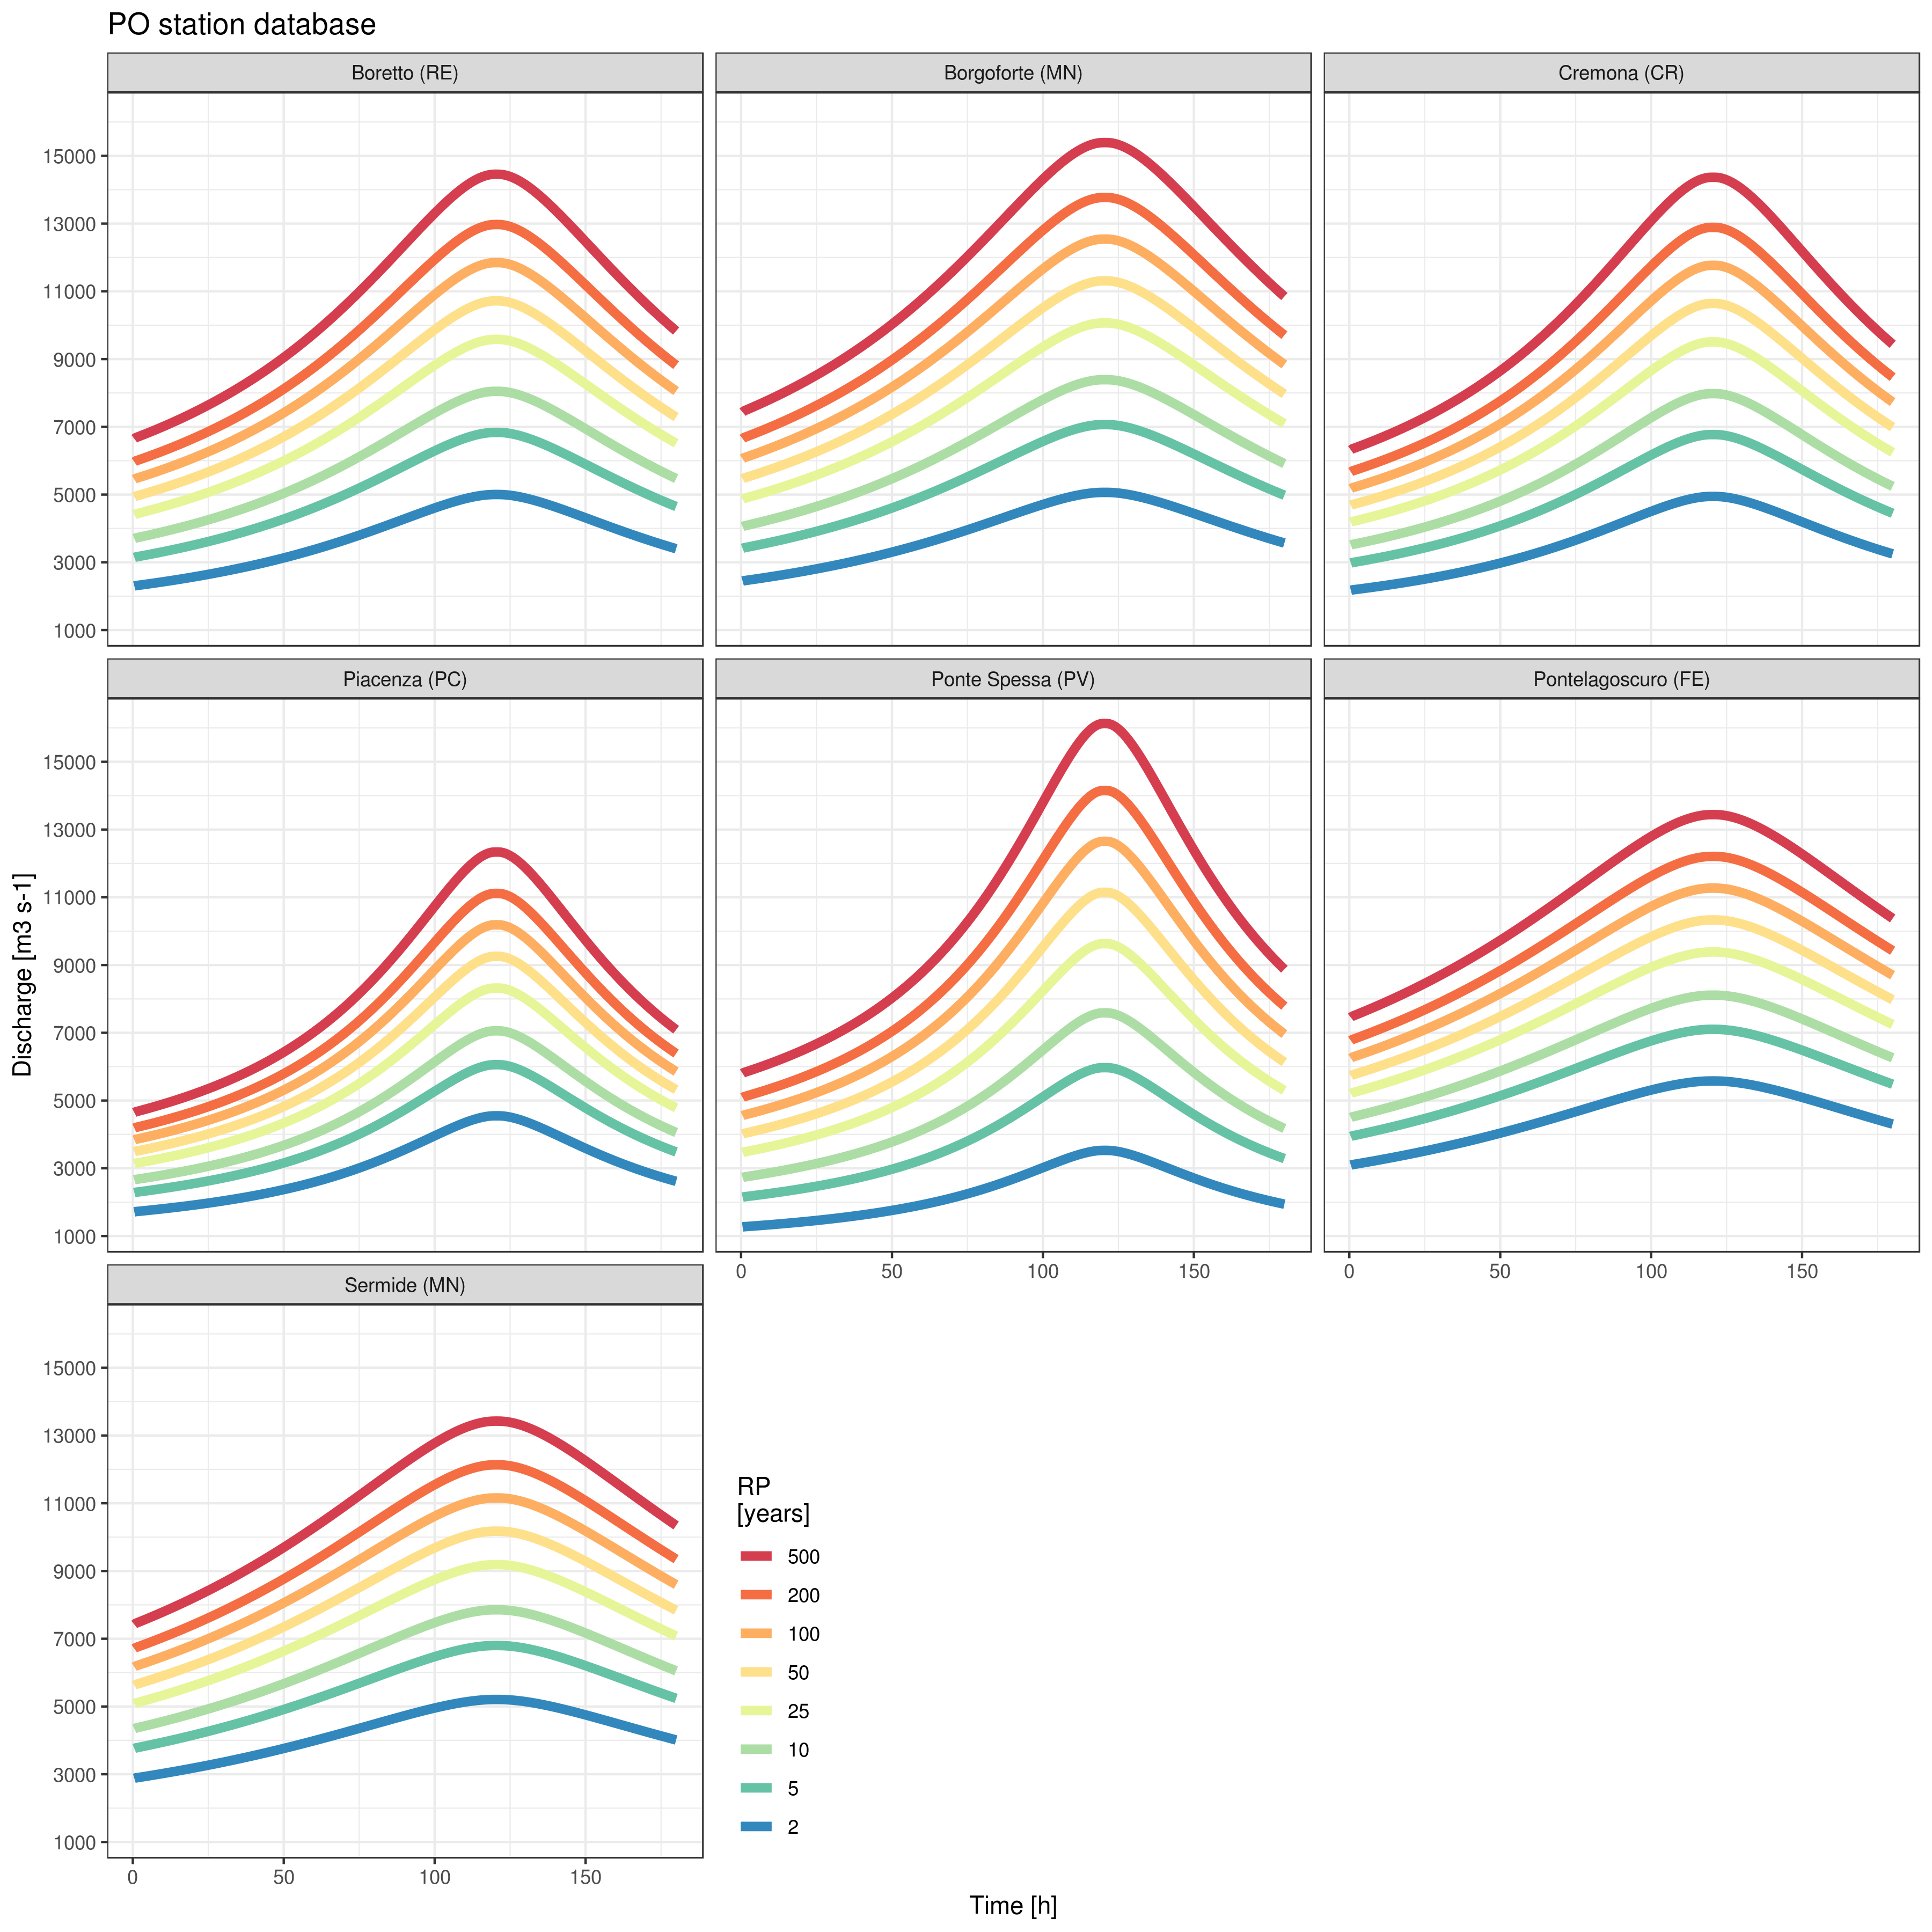
\includegraphics[width=\textwidth]{figures/valid_flood/method/po_sdh}
    \decoRule
    \caption[Synthetic Design Hydrographs for stations in the MV1 dataset]{Synthetic Design Hydrographs for the seven discharge stations in the MV1 dataset (see \cref{tab:disc_dst}), which covers the Po river; the results are in line with \citet{Maione2003}.}
    \label{fig:po_sdh}
\end{figure}


%-------------------------------
%	CA2D
%-------------------------------
\section{The CA2D hydraulic model}\label{sec:ca2d}
Floodplain hydraulic simulations are modelled with a modified version of the CA2D hydraulic model, initially introduced in \citet{Dottori2010} and described and validated in great detail in \citet{Dottori2011}.
CA2D is based on the LISFLOOD-FP model \citep{Bates2005}, a a coupled 1D/2D hydraulic model based on a raster grid which has been extensively used in flood hazard mapping \citep[see e.g.][]{ThomasStevenSavage2016, Neal2011, Skinner2015}. Instead of solving the full shallow water equations, CA2D is a reduced complexity model which uses a 2D cellular automata approach.
It is significantly faster than LISFLOOD-FP thanks to a number of optimisations and assumptions: in particular, an inertial formulation \citep{Bates2010}
for the computation of discharges and the use of a local adaptive timestep \citep{Zhang1994} enabled a \SI{97}{\%} reduction in computation time compared to LISFLOOD-FP \citep{Dottori2011}.
This makes high-resolution simulations possible even on a large scale.
The model was modified by Rita Nogherotto from the ICTP's ESP section to run in parallel, further speeding up the computation. Rita also took care of running, organising and postprocessing all of the CA2D simulations.
The model uses as input the Synthetic Design Hydrographs created starting from CHyM-simulated discharge data using the procedure described in the previous section.

A \SI{90}{\metre} resolution, corresponding to the resolution of the underlying HydroSHEDS void-filled DEM (see \cref{sec:DEM}), is selected for all simulations.
Due to its high resolution, CA2D cannot be run for the whole domain in a single simulation.
To overcome this, a large number of small scale simulations, evenly spaced along the river network, is run in parallel for each of the nine CHyM domains (see \cref{sec:chym_riv_net,fig:chym_regions}).
Each of these simulations includes exactly one ``virtual station'', which represents the water source.
Each water source itself corresponds to a specific SDH (\cref{fig:example_SHD}) generated from CHyM discharge data for the corresponding river cell.
Practical and computational considerations led to the choice of a spacing among stations varying linearly with the drained area of each point and capped between 5 and \SI{10}{\kilo\meter}.
This resulted in a total of 5548 simulations with an extent of $\ang{0.2}\times\ang{0.2}$.
The connection between CHyM's river network and CA2D's ``virtual stations'' is performed automatically with a nearest neighbour method, and is manually checked for accuracy.
This approach allowed the creation of a ensemble of small, high resolution hydraulic simulation covering the complete river network over each of the nine CHyM domains, while remaining computationally feasible; \cref{fig:ca2d_fakestations,fig:ca2d_fakestations2} show example distributions and density for the  ``virtual stations''.\\
The outputs of these small-scale simulations, once converted to netCDF, are merged together to create a large scale flood hazard map for each Return Period.
This implies an assumption of independence between simulations which, while strong, is necessary to this approach.

Further details regarding the choice of DEM, the conditioning it requires and the spacing of ``virtual station'' are provided in \citet[][in preparation]{Nogherotto2018}.
Currently, only the simulation driven by the CHyM (GRIPHO) has been completed, while other runs driven by RegCM (ERA-Interim and HadGEM) are currently ongoing.
All simulations are run on the ICTP ARGO cluster.
\begin{figure}
    \centering
    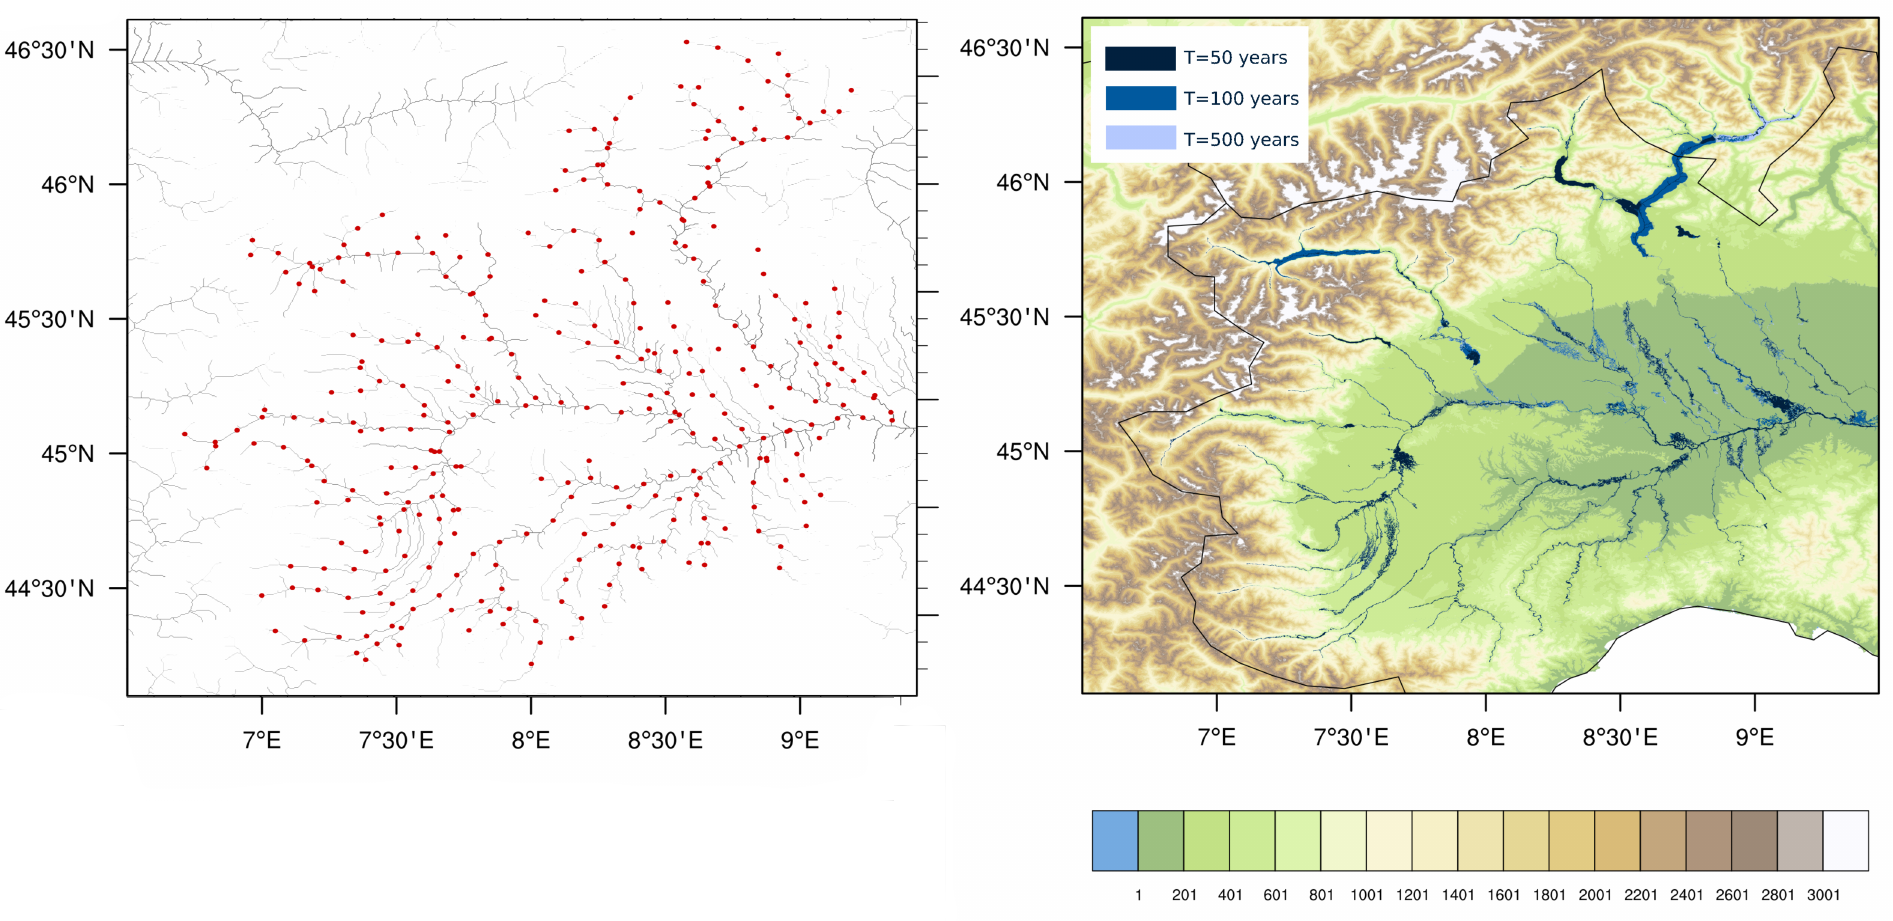
\includegraphics[width=0.9\textwidth]{figures/valid_flood/overlay_chym_locations.png}
    \decoRule
    \caption[``Virtual stations'' and preliminary results of a CA2D simulations over the upper Po basin]{``Virtual stations'' (left) and preliminary flood results (right) of a CA2D test simulation performed over the upper Po basin. From \citet{Nogherotto2018}, in preparation.}
    \label{fig:ca2d_fakestations}
\end{figure}
\begin{figure}
    \centering
    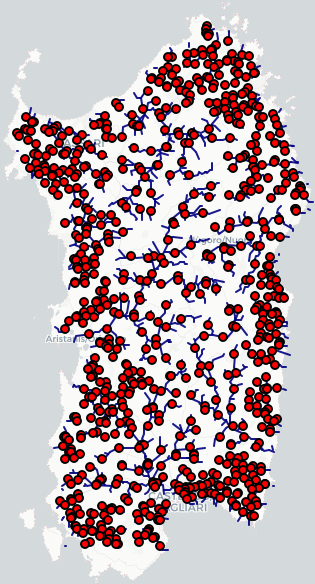
\includegraphics[width=0.5\textwidth]{figures/valid_flood/method/Sardinia}
    \decoRule
    \caption[``Virtual stations'' example over the Sardinia domain]{``Virtual stations'' (red dots) over the Sardinia domain, including river network (blue lines) for major rivers.}
    \label{fig:ca2d_fakestations2}
\end{figure}

%-------------------------------
%	TODOs
%-------------------------------
% \section{TODOs}
% \begin{itemize}
%     \item  On a smaller, catchment scale, \citet{Cloke2013} find increased flood hazard for the Upper Severn basin, but highlight potential differences when using different methodologies and models, arguing an ensemble approach would be more reliable, given the large uncertainties inherent to reproducing extreme events in a model chain. A lot of studies (e.g. Dankers2009, Alfieri2017, Kay2009, Gosling2011, Bell2007, Prudhomme2003) highlight that a multimodel ensemble is way better... I should explain why this was unattainable in our case. Rojas2012 also shows this very well.
%     \item cite \citet{Rojas2011}, it's interesting
%     \item \citet{Alfieri2015a} says (p2248) that bias correction does not help extremes, with references. Say the same!
% \end{itemize}